%============================================================================
% tento soubor pouzijte jako zaklad
% (c) 2008 Michal Bidlo
% E-mail: bidlom AT fit vutbr cz
%============================================================================
% kodovaní: iso-8859-2 (zmena prikazem iconv, recode nebo cstocs)
%----------------------------------------------------------------------------
% zpracování: make, make pdf, make desky, make clean
% připomínky posílejte na e-mail: bidlom AT fit.vutbr.cz
% vim: set syntax=tex encoding=latin2:
%============================================================================
\documentclass[cover]{fitthesis} % odevzdani do wisu - odkazy, na ktere se da klikat
%\documentclass[cover,print]{fitthesis} % pro tisk - na odkazy se neda klikat
%\documentclass[english,print]{fitthesis} % pro tisk - na odkazy se neda klikat
%      \documentclass[english]{fitthesis}
% * Je-li prace psana v anglickem jazyce, je zapotrebi u tridy pouzit 
%   parametr english nasledovne:
%      \documentclass[english]{fitthesis}
% * Neprejete-li si vysazet na prvni strane dokumentu desky, zruste 
%   parametr cover

% zde zvolime kodovani, ve kterem je napsan text prace
% "latin2" pro iso8859-2 nebo "cp1250" pro windows-1250, "utf8" pro "utf-8"
%\usepackage{ucs}
\usepackage[utf8]{inputenc}
\usepackage[T1, IL2]{fontenc}
\usepackage{url}
\usepackage{graphicx}
\usepackage{gensymb}
\DeclareUrlCommand\url{\def\UrlLeft{<}\def\UrlRight{>} \urlstyle{tt}}

%zde muzeme vlozit vlastni balicky


% =======================================================================
% balíček "hyperref" vytváří klikací odkazy v pdf, pokud tedy použijeme pdflatex
% problém je, že balíček hyperref musí být uveden jako poslední, takže nemůže
% být v šabloně
\ifWis
\ifx\pdfoutput\undefined % nejedeme pod pdflatexem
\else
  \usepackage{color}
%  \usepackage[unicode,colorlinks,hyperindex,plainpages=false,pdftex]{hyperref}
  \usepackage[unicode,colorlinks,hyperindex,plainpages=false]{hyperref}
  \definecolor{links}{rgb}{0.4,0.5,0}
  \definecolor{anchors}{rgb}{1,0,0}
  \def\AnchorColor{anchors}
  \def\LinkColor{links}
  \def\pdfBorderAttrs{/Border [0 0 0] }  % bez okrajů kolem odkazů
  \pdfcompresslevel=9
\fi
\fi

%Informace o praci/projektu
%---------------------------------------------------------------------------
\projectinfo{
  %Prace
  project=BP,            %typ prace BP/SP/DP/DR
  year=2012,             %rok
  date=\today,           %datum odevzdani
  %Nazev prace
  title.cs={HAM staniční deník pro Linux},  %nazev prace v cestine
  title.en={HAM logbook for Linux}, %nazev prace v anglictine
  %Autor
  author={Jan Kaluža},   %jmeno prijmeni autora
  %author.title.p=Bc., %titul pred jmenem (nepovinne)
  %author.title.a=PhD, %titul za jmenem (nepovinne)
  %Ustav
  department=UPSY, % doplnte prislusnou zkratku: UPSY/UIFS/UITS/UPGM
  %Skolitel
  supervisor={Václav Šimek}, %jmeno prijmeni skolitele
  supervisor.title.p=Ing.,   %titul pred jmenem (nepovinne)
%   supervisor.title.a={Ph.D.},    %titul za jmenem (nepovinne)
  %Klicova slova, abstrakty, prohlaseni a podekovani je mozne definovat 
  %bud pomoci nasledujicich parametru nebo pomoci vyhrazenych maker (viz dale)
  %===========================================================================
  %Klicova slova
  keywords.cs={HAM, amatérské radio, deník, klient, server, databáze, C++, Qt, Boost}, %klicova slova v ceskem jazyce
  keywords.en={HAM, amateur radio, logbook, client, server, database, C++, Qt, Boost}, %klicova slova v anglickem jazyce
  %Abstract
%% YARDA: Návrh abstraktu.
  abstract.cs={Cílem této bakalářské práce je návrh a implementace
  software realizujícího staniční deník amatérské radiokomunikační služby.
  Po stručném úvodu do problematiky následuje popis existujících softwarových řešení staničních deníků včetně analýzy jejich výhod a nevýhod.
  Na základě této analýzy je dále proveden návrh nového modulárního a otevřeného
  řešení, které bylo implementováno jako softwarová aplikace pro operační systém
  GNU/Linux. Zdrojové kódy byly uvolněny pod svobodnou licencí GNU GPL.
  Na závěr je provedeno zhodnocení implementace a jsou diskutovány možnosti dalšího rozšíření.
}, % abstrakt v ceskem jazyce
%% YARDA: Český návrh není přeložen.
abstract.en={The goal of this bachelor's thesis is to design and implement an
  amateur radio logbook software for a GNU/Linux operating system.
After the short introduction there are described existent logbook applications
together with analysis of their advantages and disadvantages.
Based on this analysis the logbook application is designed and implemented.
Finally, there is a summary and discussion of possibilities
for further improvements.}, % abstrakt v anglickem jazyce
  %Prohlaseni
  declaration={Prohlašuji, že jsem tuto bakalářskou práci vypracoval samostatně pod vedením pana Ing. Václava Šimka.},
  %Podekovani (nepovinne)
%   acknowledgment={Zde je možné uvést poděkování vedoucímu práce a těm, kteří poskytli odbornou pomoc.} % nepovinne
}

%Abstrakt (cesky, anglicky)
%\abstract[cs]{Do tohoto odstavce bude zapsán výtah (abstrakt) práce v českém jazyce.}
%\abstract[en]{Do tohoto odstavce bude zapsán výtah (abstrakt) práce v anglickém jazyce.}

%Klicova slova (cesky, anglicky)
%\keywords[cs]{Sem budou zapsána jednotlivá klíčová slova v českém jazyce, oddělená čárkami.}
%\keywords[en]{Sem budou zapsána jednotlivá klíčová slova v anglickém jazyce, oddělená čárkami.}

%Prohlaseni
%\declaration{Prohlašuji, že jsem tuto bakalářskou práci vypracoval samostatně pod vedením pana X...
%Další informace mi poskytli...
%Uvedl jsem všechny literární prameny a publikace, ze kterých jsem čerpal.}

%Podekovani (nepovinne)
%\acknowledgment{V této sekci je možno uvést poděkování vedoucímu práce a těm, kteří poskytli odbornou pomoc
%(externí zadavatel, konzultant, apod.).}

\begin{document}
  % Vysazeni titulnich stran
  % ----------------------------------------------
  \maketitle
  % Obsah
  % ----------------------------------------------
  \tableofcontents
  
  % Seznam obrazku a tabulek (pokud prace obsahuje velke mnozstvi obrazku, tak se to hodi)
  % \listoffigures
  % \listoftables 

  % Text prace
  % ----------------------------------------------
  \chapter{Úvod}
\label{uvod}

Cílem této práce je seznámit s oblastí radioamatérkého vysílání a se způsobem vedení staničního deníku,
zhodnotit dosavadní aplikace používané pro vedení staničního deníku a 
na základě tohoto zhodnocení vytvořit aplikaci pro vedení staničního deníku s moderní modulární architekturou,
která umožní jednoduché přidávání nových funkci.

Staniční deník je důležitou pomůckou operátora radioamatérské komunikační
služby. Slouží pro vedení záznamů o provedených spojeních.
Díky rozvoji výpočetní techniky je dnes prakticky standardem
elektronické vedení staničního deníku.
To přináší oproti klasickému papírovému deníku mnoho výhod, jež
operátorům usnadňují práci a šetří čas. Lze tak např. sledovat aktuální stav a
rozložení stanic na mapě světa, automaticky přeladit radiostanici na kmitočet
protistanice, získat detailní informace o operátorovi protistanice
prostřednictvím Internetu, rychle vyhledávat a vytvářet statistiky podle nejrůznějších kritérií a
mnohé další.

\section{Členení práce}

Tato bakalářská  práce je rozdělena do šesti kapitol.

První kapitola obsahuje úvod. Dále následuje kapitola popisující stručně historii amatérské radiokomunikační služby,
v jejíž podkapitolách jsou rovněž vysvětleny důležíté pojmy a popsány služby používané radioamatéry.
Třetí kapitola popisuje současný stav, jsou krátce představeny existující
aplikace pro vedení staničních deníků včetně jejich výhod a nevýhod. V
následující čtvrté kapitole je proveden analýza a jsou navrženy jednotlivé části staničního deníku.
Pátá kapitola pojednává a implementaci. V šesté kapitole je zmíněn jednoduchý příklad použití výsledné aplikace
 a v poslední šesté kapitole je práce zhodnocena a jsou zmíněny možnosti jejího
 dalšího rozšíření.


%% YARDA: Pojmenoval bych amatérská radiokomunikační služba, dále v textu bych vysvětlil
%% právní status, např. z ČRK:
%% YARDA (DONE): mám trochu problém se slovem rádio, podle mě je to slangový výraz
%% pro radiopřijímač, proto např. na webu ČRK se spojení 'amatérské rádio'
%% poměrně úspěšně vyhýbají :) Přestože spojení 'amatérské rádio' se u nás
%% poměrně dost často používá, asi bych se mu taky radši vyhnul a místo toho použil např.
%% 'amatérské vysílání' nebo 'HAM radio', případně
%% 'amatérské radio' viz např. časopis Amatérské radio (http://www.aradio.cz/)
%% I když toto je spíš otázka pro nějakého etymologa :)

\chapter{Amatérská radiokomunikační služba}
\label{radioamateri}

V této kapitole je definována amatérská radiokomunikační služba, dále je stručně popsána historie amatérského vysílání a jsou zde vysvětleny důležité pojmy používané dále v práci. Informace byly převzaty zejména z \cite{crk_hist}.

\section{Definice}
\label{radioamateri_def}

Radiokomunikační řád definuje amatérskou službu jako
radiokomunikační službu, která slouží k vlastnímu vzdělávání, vzájemné
komunikaci a technickému zkoumání uskutečňovanému amatéry, to je plně
autorizovanými osobami, které se zajímají o radiotechniku jedině z osobního
snažení a bez peněžních zájmů. Obdobně je definována i amatérská družicová
služba, která k radiové komunikaci používá vesmírné stanice na družicích.

Radiokomunikační řád je jedním ze základních dokumentů Mezinárodní
telekomunikační unie (anglicky International telecommunication union, dále jen
ITU). %% YARDA2: link na stranky ITU www.itu.int
ITU byla založena již 17.května 1865 dvaceti evropskými státy, tehdy pod názvem Mezinárodní telegrafní
unie. Naše země stála u jejího zrodu ještě jako součást rakouského mocnářství. ITU
je dnes stálou mezinárodní organizací při OSN pro dálkové telekomunikace a
správu kmitočtového spektra.
Opatření ITU jsou v ČR právně závazná z titulu členství ČR v ITU a v
mezích základních dokumentů ITU. O národní koordinaci se v ČR stará
Český telekomunikační úřad (ČTÚ). %% YARDA2: link na ČTÚ www.ctu.cz
%% YARDA2: radiokomunikační řád je k dispozici k zakoupení na stránkách ITU:
%% http://www.itu.int/pub/R-REG-RR-2004, dal bych to jako poznámku pod čarou

%% YARDA2: nazev kapitoly bych zkratil na historie
\section{Historie}
\label{radioamateri_hist}
Prvotní motivací pro vznik amatérského vysílání %% YARDA (DONE): Tady bych dal např. amatérského vysílaní atd.
byla myšlenka našich předků radio %% YARDA (DONE): Asi radio jako mají na ČRK.
nejen poslouchat, ale také nezávisle vysílat.
To dalo vzniknout novému druhu zábavy - amatérskému vysílání (HAM Radio). Lidem, kteří vysílali se pak začalo říkat 
radioamatéři.

Amatérské vysílání se začalo rychle šířit po první světové válce hlavně díky vlivu
rozhlasu. %% YARDA (DONE): tady bych byl konzistentní v pojmech, komerční radiové
%% vysílání jako rozhlas (AFAIK původně vzniklo ze slova radiožurnál) vs v
%% dřívějším odstavci 'radio' pro označení toho stejného.
V těchto dobách radioamatéři značně
přispěli k získání znalostí o využití celého spektra radiových vln. Vysílali na dlouhých a středních vlnách, které byly do té doby
považovány za bezcenné, a také na vlnách krátkých, o jejichž existenci se nevědělo vůbec.
%% YARDA (DONE): Přidat následující (důležité):
%% Když Marconi poprvé propojil radiem Evropu a Ameriku, potřeboval na dlouhých
%% vlnách mnoho kilowattů výkonu a kilometrové antény. V roce 1923 radioamatéři
%% zjistili, že na krátkých vlnách jim k témuž stačí energie jedné žárovky a pár
%% desítek metrů drátu jako anténa. To odstartovalo následné komerční využivání
%% těchto pásem.

Na dlouhých vlnách potřeboval například Marconi mnoho kilowattů výkonu a kilometrové antény pro první spojení
mezi Evropou a Amerikou. Oproti tomu stačila radioamatérům v roce 1923 díky využití krátkých vln
pro stejné spojení jen energie jedné žárovky a anténa o velikosti pár desítek
metrů. To odstartovalo další komerční
využívání těchto pásem.

První pokusy o transatlantické spojení začaly lákat také Pravoslava Motyčku - prvního známého radioamatéra u nás.
Koncem roku 1924 navázal Motyčka první spojení v Československu. 
Díky Motyčkově inspiraci bylo u nás kolem 30. let 20. století až několik set radioamatérů.

Dalším významným rokem byl rok 1928, kdy byl ruský radioamatér prvním, kdo zachytil volání vzducholodi ITALIA,
která ztroskotala na cestě od severního pólu. To změnilo pohled na amatérské
rádio, do té doby vnímané spíše jako zábava. Při mnoha pohromách na celém světě
pak pomáhala připravenost radioamatérů poskytnout spojení do
jiných míst.

\section{Amatérské vysílání dnes}
\label{radioamateri_dnes}

Radioamatéři jsou aktivní prakticky na všech pásmech, pracují s analogovými i
digitálními druhy provozů, využívají moderní technologii jako např. spojení přes
převaděče na nízkoorbitálních satelitech, vesmírné stanicii ISS, atp. 

Za základní pilíř radioamatérského snažení lze však stále považovat vysílání na
krátkých vlnách, jež umožňuje spojení do celého světa včetně exotických zemí. K
tomu se nejčastěji využívá šíření vln odrazem od různých vrstev ionosféry.

Řada radioamatérů se snaží o co nejdelší spojení s co nejvíce exotickými zeměmi.
Tato aktivita se obecně nazývá DX provoz neboli DXing. Zkratka DX je původně souhrné pojmenování
pro dálkový příjem/vysílání. Pochází z anglického "distance
x", neboli vzdálenost neznámá. V současné době radioamatéři pod pojmem DX
nejčastěji rozumí mezikontinentální spojení.
Po úspěšně navázaném spojení si radioamatéři vyměnují QSL lístky (písemné potvrzení o
navázaném spojení ve formátu pohlednice). Nepsaným pravidlem je výměna QSL
lístků při prvním spojení s novou stanicí. Jedním z cílů tohoto snažení je
získání QSL lístků z co možná nejvíce zemí světa (ideálně všech).

U profesionálního komerčního vysílání (například FM rozhlas nebo
televize) je třeba pro dosažení kvalitního příjmu být od vysílače vzdálen maximálně
v desítkách kilometrů. Tyto služby jsou navrženy pro stabilní pokrytí určité
oblasti v definované kvalitě. Radioamatérům však nejde o profesionální kvalitu.
Důležitější je úspěšné navázání spojení. Radioamatáři se neustále snaží o překonávání limitů.
Pokud se jim například podaří uskutečnit spojení na jednom pásmu,
snaží se o totéž i na dalších pásmech, jež však nemusí být za daných
podmínek pro spojení nejvhodnější a například komerční služby by o takovém
použití vůbec neuvažovaly.

K navázání spojení radioamatéři využívají kromě
kvalitní techniky také dobrých znalostí faktorů
ovliňujících šíření krátkých vln. Těmi jsou např. sluneční aktivita,
stav ionosféry, denní a roční doba a taktéž aktuální meteorologické podmínky
jako například výskyt
rozhraní teplých a studených mas vzduchu. Využívají se i znalosti o výskytu
meteoritických rojů nebo polárních září. Profesionálové se nemohou na tyto přechodné faktory spolehnout, ale 
radioamatéři jsou díky nim schopni navázat spojení prakticky po celém světě.
Radioamatéři pracující na krátkých vlnách jsou nezávislí na externí
infrastruktuře. O jejich úspěšnosti či neúspěšnosti rozhoduje kvalita použité techniky,
jejich znalosti a schopnosti, kvalita použitých anténních systémů a příroda. Nezávislost na externí infrastruktuře je velkou výhodou např. v
případě živelních pohrom. V těchto krizových situacích, kdy jsou často veřejné
komunikační sítě vyřazeny z provozu, jsou radioamáteři schopni poskytovat
spojení s okolním světem a předávat informace nezbytné pro řízení záchraných
operací. V tomto směru se radioamatéři v poslední době pozitivně vyznamenali
např. při nedávných neštěstích v Japonsku a v Thajsku. 

Další radioamatérskou aktivitou je práce na VKV/UKV (neboli velmi krátkých/ultra
krátkých vlnách). Tato spojení se vyznačují mnohem vyšší kvalitou srovnatelnou s
profesionálními službami, nicméně pro jejich navázání je třeba přímá radiová
viditelnost mezi jednotlivými stanicemi (v praxi je přímá radiová viditelnost
většinou srovnatelná nebo díky odrazům a lomům trochu vyšší než přímá optická
viditelnost).
Z toho důvodu se na řadu vysokých budov a kopců umisťují tzv. pozemní rádiové
převaděče. Převaděč přijímá signál na jedné frekvenci, zesiluje ho a přeposílá
dále na frekvenci jiné. Díky tomu lze spolehlivě pokrýt oblasti jako města či kraje.
Dalším častým vylepšením je propojování těchto převaděčů do sítí. Díky tomu mohou
radioamatéři navazovat spojení i se stanicemi nacházejícími se v dosahu
propojených převaděčů. Velice oblíbený v tomto směru je např. systém
Echolink \cite{echolink}, %%YARDA (DONE): link literatura, na echolink.org,
který umožňuje celosvětově vytvářet tzv. červí díry (wormholes) mezi libovolnými
převaděči v této síti.

Příklad použití: stanice v dosahu brněnského převaděče
zadá kód 366111, což zajistí propojení s převaděčem v Honolulu (propojení je
nejčastěji realizováno pomocí sítě Internet). Radioamatéři se tak mohou pomocí převaděče dovolat na velké vzdálenosti i s použitím vysílačů o malém výkonu
(často jde o kapesní radiostanice o velikosti srovnatelné s mobilním telefonem).
Jistou daní je však závislost na externí infrastruktuře, což komplikuje využití
této technologie v případě krizových situací.

V počátcích 60. let byl také vypuštěn první radioamatérský satelit. Dnes jich existuje několik desítek.
Tato činnost je koordinována neziskovou organizací AMSAT \cite{amsat}. %% YARDA: link na AMSAT %% YARDA (DONE): konzistentní terminologie, družice vs satelit
Narozdíl od geostacionárních družic, které šíří např. televizní
signál a jsou tzv. zaparkovány na vysokých oběžných drahách, však amatérské
družice kolem Země obíhají na nízkých oběžných drahách (tzv. LEO - Low Earth
orbit). %% YARDA: může být link
Díky tomu jsou schopny pokrýt postupně signálem všechny obydlené oblasti.

Radioamatéři rovněž pořádají závody. Cílem je například v určitém čase navázat spojení s co nejvíce jinými
amatérskými stanicemi v co nejvíce zemích. Jinou variantou je například součet vzdáleností všech spojení vykonaných za určitý
čas. Jednotlivé závody mají svoje definovaná pravidla a jsou vypisovány pro
různé kategorie.

K radioamatérům neodmyslitelně patří Morseova abeceda. Morseova abeceda byla
prvním dorozumívacím prostředkem a je radioamatéry používána dodnes.
Výhodou Morseovy %% YARDA (DONE): asi bych dal velké M
abecedy je její velká odolnost proti rušení, diký níž lze překonat velké vzdálenosti i s malým
výkonem. Taktéž pro její příjem a vysílání stačí principiálně jednoduchá
zařízení. Další výhodou je to, že odbourává
jazykové bariéry, protože se v ní komunikuje
převážně pomocí krátkých mezinárodních kódů (tzv. Q kódy). Při hlasové komunikaci
je mezinárodním jazykem angličtina (pokud však protistanice rozumí, lze pro
spojení použít i libovolný jiný jazyk) a využívá se nejčastěji amplitudové
modulace s potlačeným postraním pásmem SSB
nebo FM modulace. Nejnověji se experimentuje i s různými digitálními režimy
přenosu hlasu, např. D-STAR, %% YARDA (DONE): link
P25 C4FM, atp.

Historicky se však digitálně přenášely jen data o malém objemu a původně jen nízkou
přenosovou rychlostí. S postupným vývojem však dochází k nárůstu přenosové
rychlosti. Tyto systémy přenosu dat se nazývají Packet radio. V podstatě se jedná o
radioamatérský Internet, kde se informace přenáší pomocí modifikace protokolu
X.25 (tzv. AX.25) \cite{ax25}. %% YARDA (DONE): link 
Jednotlivé uzly sítě jsou vzájemně propojeny (většinou radiovou cestou, nověji i
přes Internet) a pakety putují přes jednotlivé uzly.
Síť packet radia pokrývá celý vyspělý svět, její součástí jsou i BBS (Bulletin
board system - databanky pro ukládání a výměnu informací) a
elektronická pošta. Poslat e-mail kamarádovi do Austrálie tedy nemusíme jen po Internetu,
ale také amatérským packet radiem, případně lze trávit hodiny zkoumáním nových zpráv i
zajímavých programů v desítkách BBS.

Lze vysílat i obrazové signály. Dlouhou tradici má tzv. pomalá televize (Slow
    scan TV - SSTV),
jaká byla použita i u přenosu obrazu z prvních přistání amerických astronautů na Měsíci,
dnes se experimentuje s různými digitálními přenosy a na UHF kmitočtech je možné
použít i klasickou televizní normu.

Z ryze sportovních aktivit je dobře známý rádiový
orientační běh (ROB). Cílem je v nejkratším čase najít pomocí
přijímače v terénu ukryté zamaskované vysílače. 
Tyto sporty jsou atraktivní a pěstují je i lidé, kteří se jinak o radioamatérství příliš nezajímají.

Z dalších aktivit radioamatérů jistě zaslouží zmínku EME (Earth Moon Earth), kdy
se navazují spojení odrazem od měsíce. Tato aktivita se v poslední době těší čím
dál tím vyšší oblibě. Vzhledem k vysokým ztrátám této přenosové cesty se
většinou komunikuje hluboko pod úrovní šumu pomocí digitálního režimu WSJT.
%% YARDA2: možná link http://physics.princeton.edu/pulsar/K1JT/

Zajímavou oblastí jsou i experimenty v oblasti mikrovln, kde jsou radioamatéři
držiteli řady světových rekordů. 

Tato podkapitola byla pokusem o stručný popis nejrozšířenějších činnosti v současnosti provozovaných
radioamatéry. Rozhodně zde nebyly popsány všechny činnosti, protože to by si
vyžádalo několikanásobně více prostoru.

\section{Staniční deník}
\label{stanicni_denik}

V této podkapitole je stručně popsán staniční deník a také údaje do něj zapisované.
Při popisu jednotlivých údajů v této kapitole se vychází z \cite{pozadavky}.

Dle §5 Vyhlášky o technických a provozních podmínkách amatérské radiokomunikační služby \cite{vyhlaska}
mají klubové stanice povinnost vést staniční deník a ukládat do něj zejména tyto údaje: datum, čas a dobu trvání
uskutečněného rádiového spojení, použité kmitočtové pásmo, druh provozu,
volací značku stanice a stanoviště klubové stanice, se kterou bylo uskutečněno rádiové spojení.

Ačkoliv je tato povinnost nyní stanovena pouze pro klubové stanice (předchozí
vyhláška ji stanovovala pro všechny stanice), většina radioamatérů si vede
elektronický staniční deník kvůli přehledu, statistikám a
vyřizování QSL agendy.

Staniční deník si lze představit jako databázi spojení provedených operátorem dané stanice.
Kromě základních údajů definovaných výše zmíněnou vyhláškou se do staničních deníků ukládají i další údaje
nad její rámec. V následující části jsou tyto jednotlivé údaje popsány a vysvětleny.

Obrázky použité dále v této podkapitole byly získány z \cite{mapability}.

\subsection{Volací značka}

Každá stanice má přidělenu jedinečnou volací značku, kterou operátor stanice uvádí při každém spojení.
První dva znaky (někdy méně) značky jsou většinou určeny podle přehledu mezinárodních volacích znaků
přidělených dané zemi.
Dalším znakem je číslice 0-9. Kombinaci těchto znaků se říká prefix (většinou 1 až
3 znaky). Zbytek značky je tvořen jedním až čtyřmi znaky.

Na základě prefixu tak lze určit zemi, ze které daný operátor pochází a tak i
jeho přibližnou polohu. K tomu slouží seznam DXCC (DX Century Club) \cite{dxcc} %% YARDA (DONE): link
obsahující všechny aktuálně používané prefixy a informace k nim.

\subsection{Druh provozu}

Na jednom kmitočtu může být spojení uskutečněno různými druhy provozu. Pro
úspěšné navázání spojení je tedy nutné, aby obě stanice použily stejný kmitočet
a stejný druh provozu. Analogové druhy provozu jsou například: telegrafie (CW), frekvenční modulace (FM), amplitudová modulace (AM),
amplitudová modulace s jedním potlačeným postraním pásmem (SSB). Digitální druhy provozu jsou například: RTTY, AMTOR, PACTOR, PSK, WSJT, D-Star, P-25, atd.

Aby nedocházalo k vzájemnému rušení je pásmo rozděleno na jednotlivé úseky s
definovaným využitím (např. kmitočty pro telegrafii, kmitočty přednostně určené
pro mezinárodní spojení, atp.). Toto rozdělení definuje kmitočtový plán (pro KV
k dispozci např. na \cite{plan_kv}, pro VKV k dispozici např. na
\cite{plan_kv}).

\subsection{ITU zóny}

Lokalizace protistanice je velmi důležitá, protože nám umožňuje zjistit, jak
daleko jsme se vlastně dovolali. V dnešní době tak rozšířené GPS, na toto není
úplně nejvhodnější, protože telegrafický přenos velkého množství číslic
by nebyl praktický a mohlo by docházet ke zbytečným chybám. Z tohoto důvodu se
používají různé jiné systémy rozdělení světa. Jedním z nich je rozdělení do takzvaných ITU zón.
Toto rozdělení lze vidět na obrázku \ref{fig:itu_zony}.
Systém je pojmenován podle organizace ITU (viz úvodní kapitola). Svět je rozdělen do celkem 
89 zón ve třech regionech.

\begin{figure}[h]
\centering
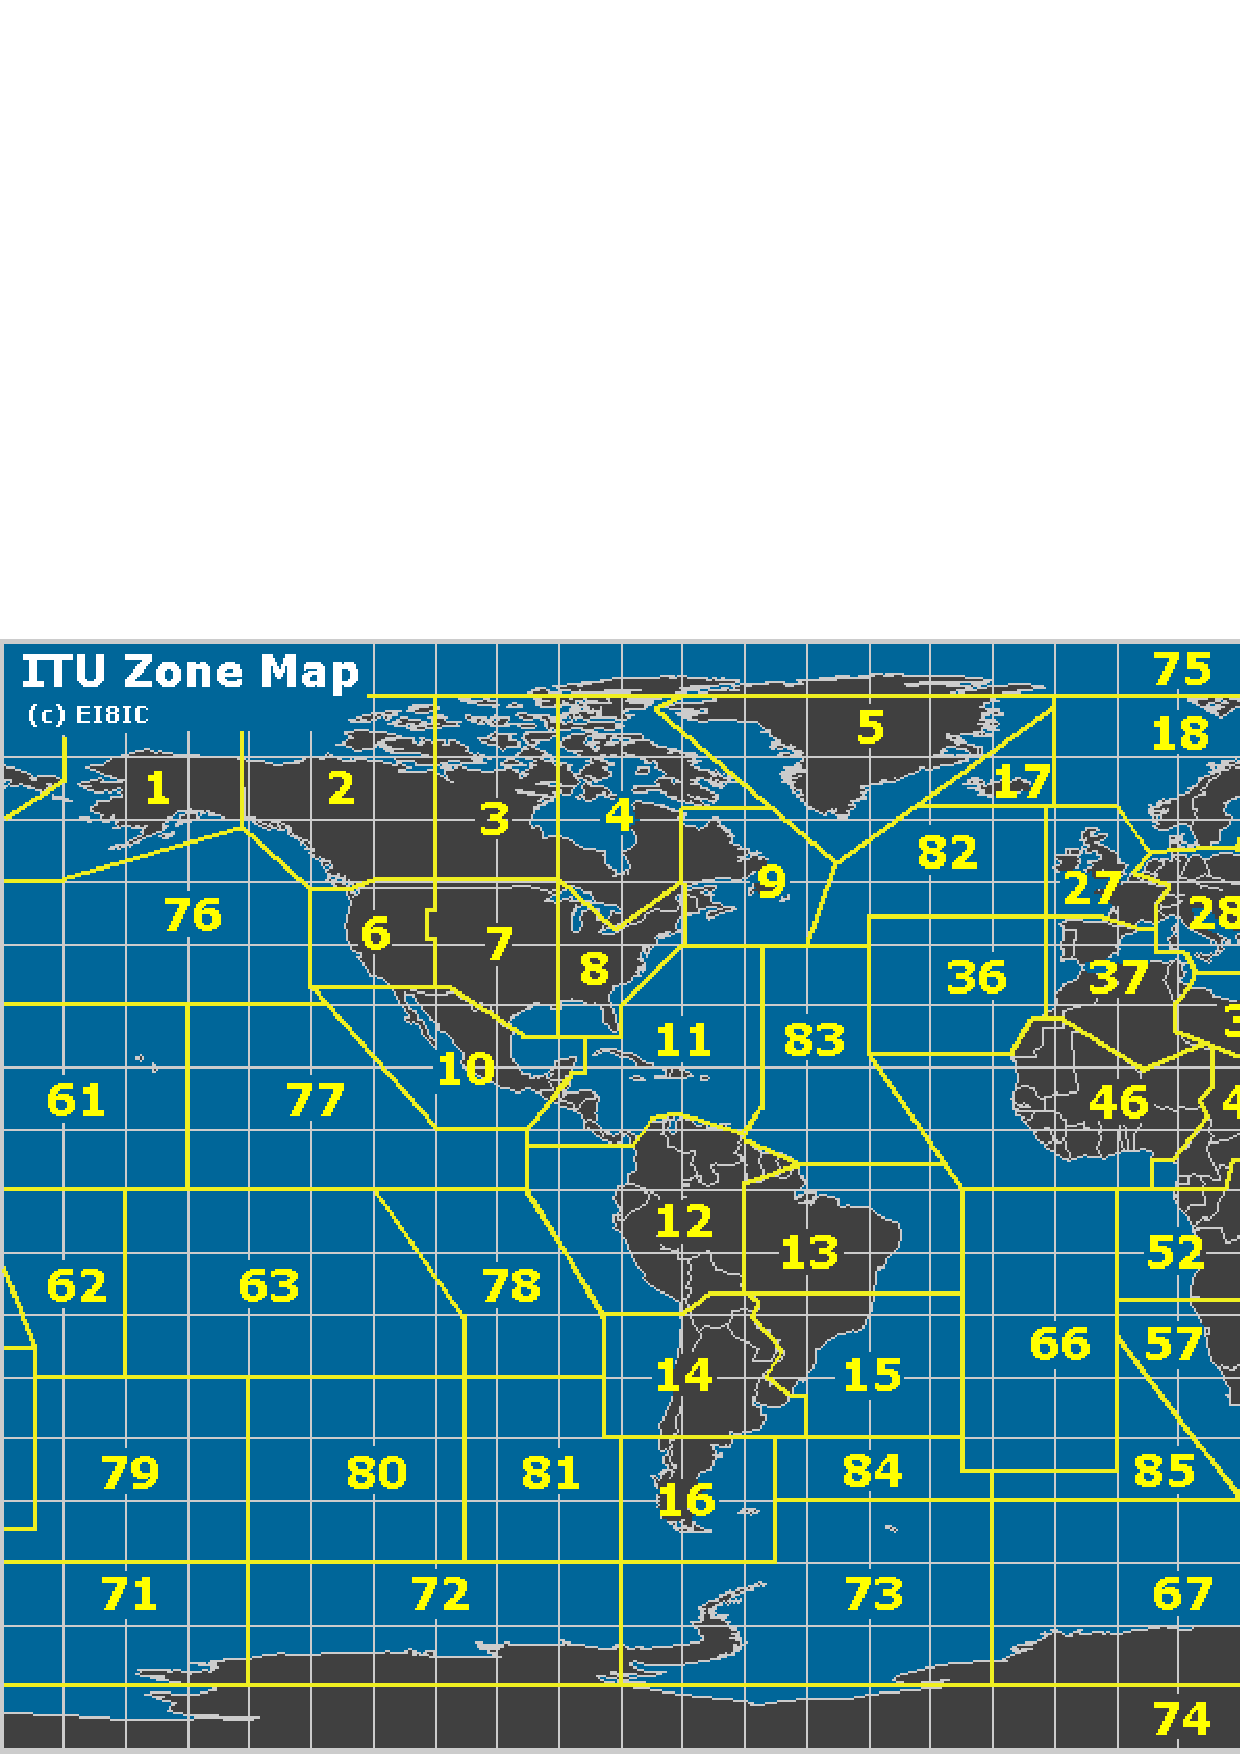
\includegraphics[trim=0cm 0cm 0cm 0cm, scale=0.4]{fig/itu-zone}
\caption{Rozdělení ITU zón.}
\label{fig:itu_zony}
\end{figure}

\subsection{CQ zóny}

Dalším z možných rozdělení světa používaných radioamatéry je dělení na CQ zóny, pojmenované podle časopisu CQ.
jak je zřejmé z obrázku \ref{fig:cq_zony}, jde o pouze 40 zón.

\begin{figure}[h]
\centering
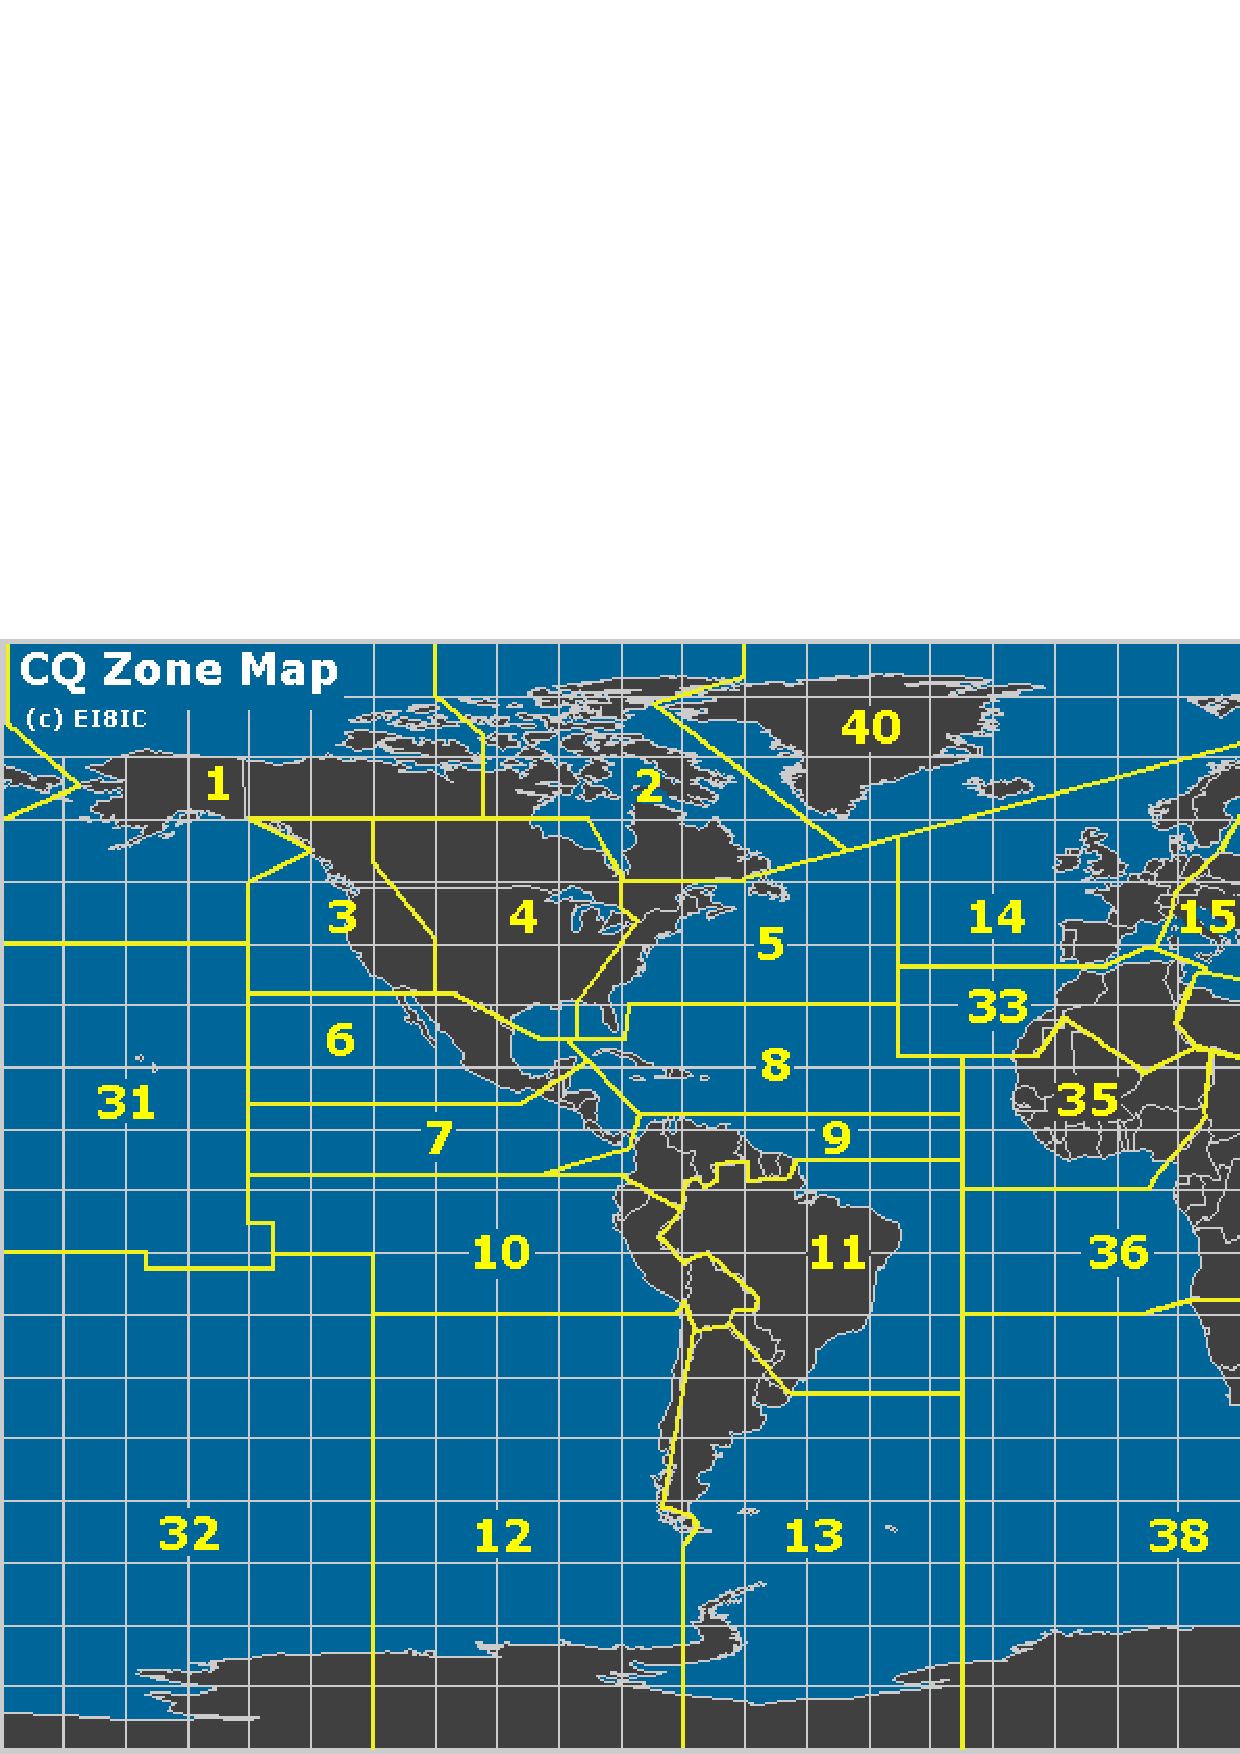
\includegraphics[trim=0cm 0cm 0cm 0cm, scale=0.4]{fig/cq-zone}
\caption{Rozdělení CQ zón.}
\label{fig:cq_zony}
\end{figure}

\subsection{QTH lokátor}

Poslední z používaných systémů pro rozdělení světa je QTH lokátor. Jde o rozdělení na základě zeměpisné šířky a délky.
Země je rozdělena do obdélníků o velikosti 1\degree x 2\degree (tzv. velký
čtverec). Ty lze hierarchicky dělit na menší obdélníky. Vzniká tak hierarchický
souřadnicový systém tvořený 2-8 znaky/číslicemi, jehož výhodou  oproti GPS
souřadnicím je, že stačí zachytit např. jen první dva znaky a známe přibližnou
polohu protistanice. Další znaky pak slouží ke zpřesnění polohy. Nejčastěji se
mezi radioamatéry používá 4 (na KV) nebo 6 (na VKV) znaků, např. JN89GE označuje
západní Brno. Toto rozdělení je zobrazeno na obrázku \ref{fig:qth}

\begin{figure}[h]
\centering
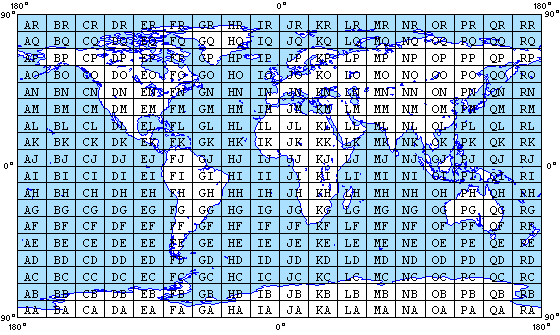
\includegraphics[trim=0cm 0cm 0cm 0cm, scale=0.7]{fig/QTH_locator}
\caption{Mapa rozdělení pomocí QTH lokátoru.}
\label{fig:qth}
\end{figure}

\subsection{Systém RST}

Důležitým údajem, který si stanice navzájem sdělují, je kvalita přijatého
signálu. V praxi se pro toto používá systém RST. Výměna RST reportu je nezbytným předpokladem platnosti radioamatérského spojení.
Název systému RST je tvořen iniciálami veličin, které obsahuje: Readability (čitelnost), Strenght (síla), Tone (tón).
RT se určuje pouze sluchem (vyžaduje určitý cvik), S se odečítá z měřiče síly
signálu (tzv. S-meter).
Při telegrafii se používá systému RST, při analogovém přenosu řeči se používá
pouze systému RS, při digitálním přenosu se používá systému RSQ (Readability, Strenght, Quality).

Každá veličina se udává pomocí číslice z intervalu 1 - 9 (čitelnost z intervalu 1 - 5), kde nejnižšímu číslu odpovídá nejnižší kvalita.
Maximálně nejlepší report v systému RST je vyjádřen údajem 599, v systému RS údajem 59.

Slovní popis jednotlivých hodnot veličin RST pro analogové a digitální módy zde z kapacitních důvodů není zmíněn, lze jej však
nalézt na stránkách Českého Radioklubu \cite{crk_rst}.

\subsection{Informace o výměně QSL lístků}

Jak již bylo zmíněno v kapitole \ref{radioamateri_dnes}, po úspěšně navázaném spojení si radioamatéři vyměnují QSL lístky.
Jedná se o kartičky podobné pohlednicím. QSL lístek obsahuje především nejzákladnější informace o operátorovi.
Jde hlavně o jeho značku, zemi, umístění stanice včetně zařazení do zón a lokátoru.
Musí také obsahovat značku protistanice, datum a čas navázání spojení, kmitočet, druh modulace a report v systému RST. 

Ve staničním deníku je pak vhodné u konkrétního spojení uchovávat informaci o tom, jestli operátor již poslal druhé
straně QSL lístek a jestli již od druhé strany QSL lístek obdržel.


\section{Služby používané radioamatéry}
\label{radioamateri_sluzby}

Díky rozšiřování Internetu se začaly rozvíjet i služby provozované radioamatéry pro další radioamatéry. V této podkapitole
jsou stručně popsány online služby, které jsou v navrhovaném staničním deníku využity.

\subsection{DXCluster}

DXCluster je komunitní službou umožňující radioamatérovi informovat ostatní
radioamatéry o tom, kdo, kde a odkud aktuálně vysílá. Díky této službě tak lze jednodušeji navazovat
spojení. Protokol služby DXCluster je v Internetu postaven na službě telnet a není nikterak
složitý. Lze jej jednoduše číst a zpracovávat. Tato služba byla historicky
šířena přes Packet radio, ale v současné době se k ní lze pohodlně připojit i přes
Internet.

\subsection{QRZ.com}

QRZ.com je v současnosti asi největší online databází radioamatérů z celého světa. Na základě volací značky lze s její pomocí zjistit detailní
informace (například jméno nebo přesnou polohu) o jejím majiteli. Vyhledávat lze i pomocí speciálního webového rozhraní
postaveného na technologii XML. To je velmi výhodné pro tvorbu aplikací využívajících QRZ.com pro zjištění informací o
operátorech.

\chapter{Současný stav}
\label{soucasnost}

V této kapitole jsou popsány existující softwarové staniční deníky. Každá aplikace je stručně
popsána a jsou zmíněny i její klady a zápory. Na základě této kapitoly bude dále
vytvořen vlastní návrh staničního deníku.

\section{Logger32}%% YARDA (DONE): logovací aplikace nahradit staniční deník

Logger32 je jedním z nejznámějších staničních deníků pro operační systém Windows. Jeho hlavní výhodou je přehledné a funkční
uživatelské rozhraní (viz obrázek \ref{fig:logger32}), které poskytuje pokročilé možnosti přizpůsobení a podpora přídavných pluginů.

\begin{figure}[h]
\centering
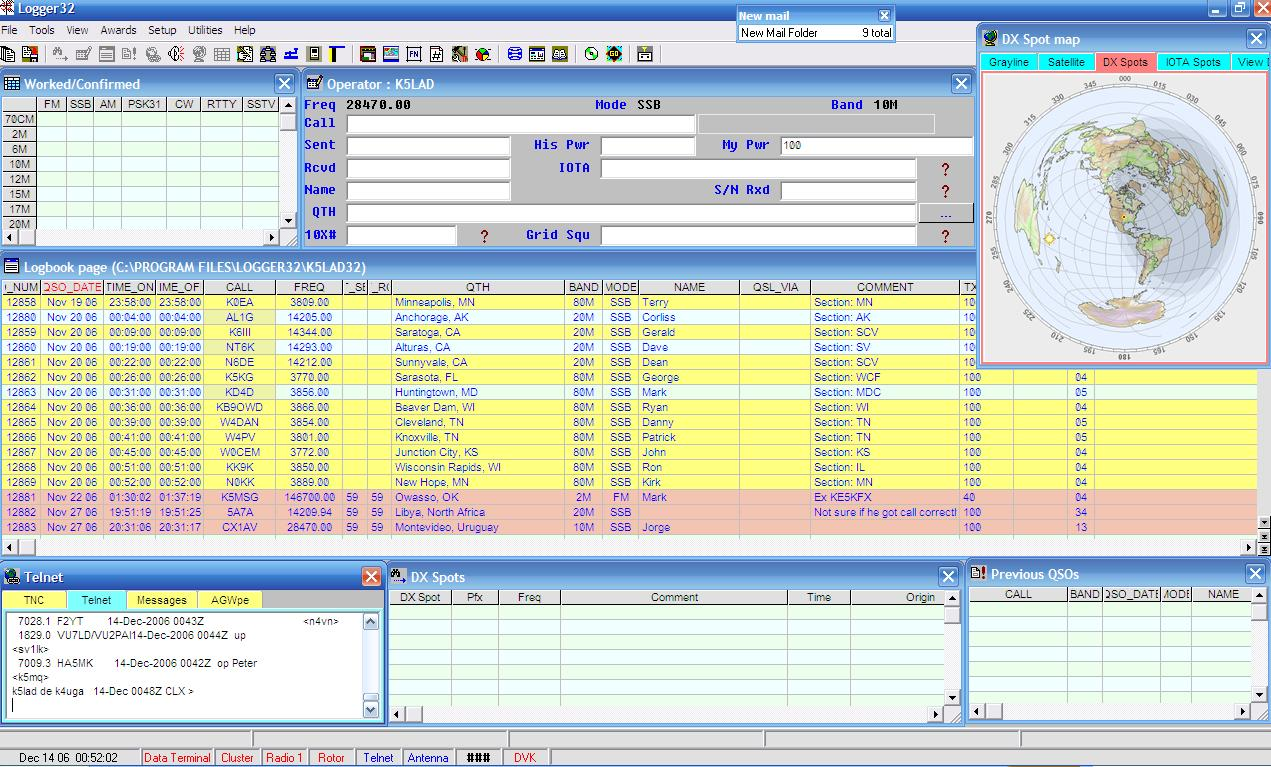
\includegraphics[trim=0cm 0cm 0cm 0cm, scale=0.33]{fig/logger32}
\caption{Uživatelské rozhraní Logger32.}
\label{fig:logger32}
\end{figure}

Lze vytvářet pluginy pro vyhledávání detailních informací na základě volací značky a také pluginy vytvářející externí okno
s rozšiřujícími informacemi. Logger32 také umožňuje dálkové ovládání
radiostanice a příslušenství. Jeho velkou výhodou je univerzálnost.

Hlavní nevýhodou aplikace Logger32 je její závislost na systému Windows. Další nevýhodou je absence zdrojových kódů, takže je rozšířitelnost aplikace limitována rozhraním modulů definovaným
tvůrcem aplikace. Nevýhodou je též implementace v jazyce Visual Basic
(výkonostní problémy).
Taktéž pro ukládání dat nelze použít externí databázi jako například SQLite3
nebo MySQL. Problémem může být rovněž nemožnost přistupovat do databáze jiným
způsobem, např. není možné řešit situaci, kdy by uživatel potřeboval z terénu 
zapsat %% YARDA (DONE): místo zalogovat používat např. zapsat
nové spojení z mobilního telefonu nebo jiného zařízení s nestandardním operačním systémem.

\section{CQRLOG}

CQRLOG je nejpoužívanějším staničním deníkem z řad multiplatformních aplikací. Je možné jej používat jak v systému
Windows, tak v Linuxových distribucích.

\begin{figure}[h]
\centering
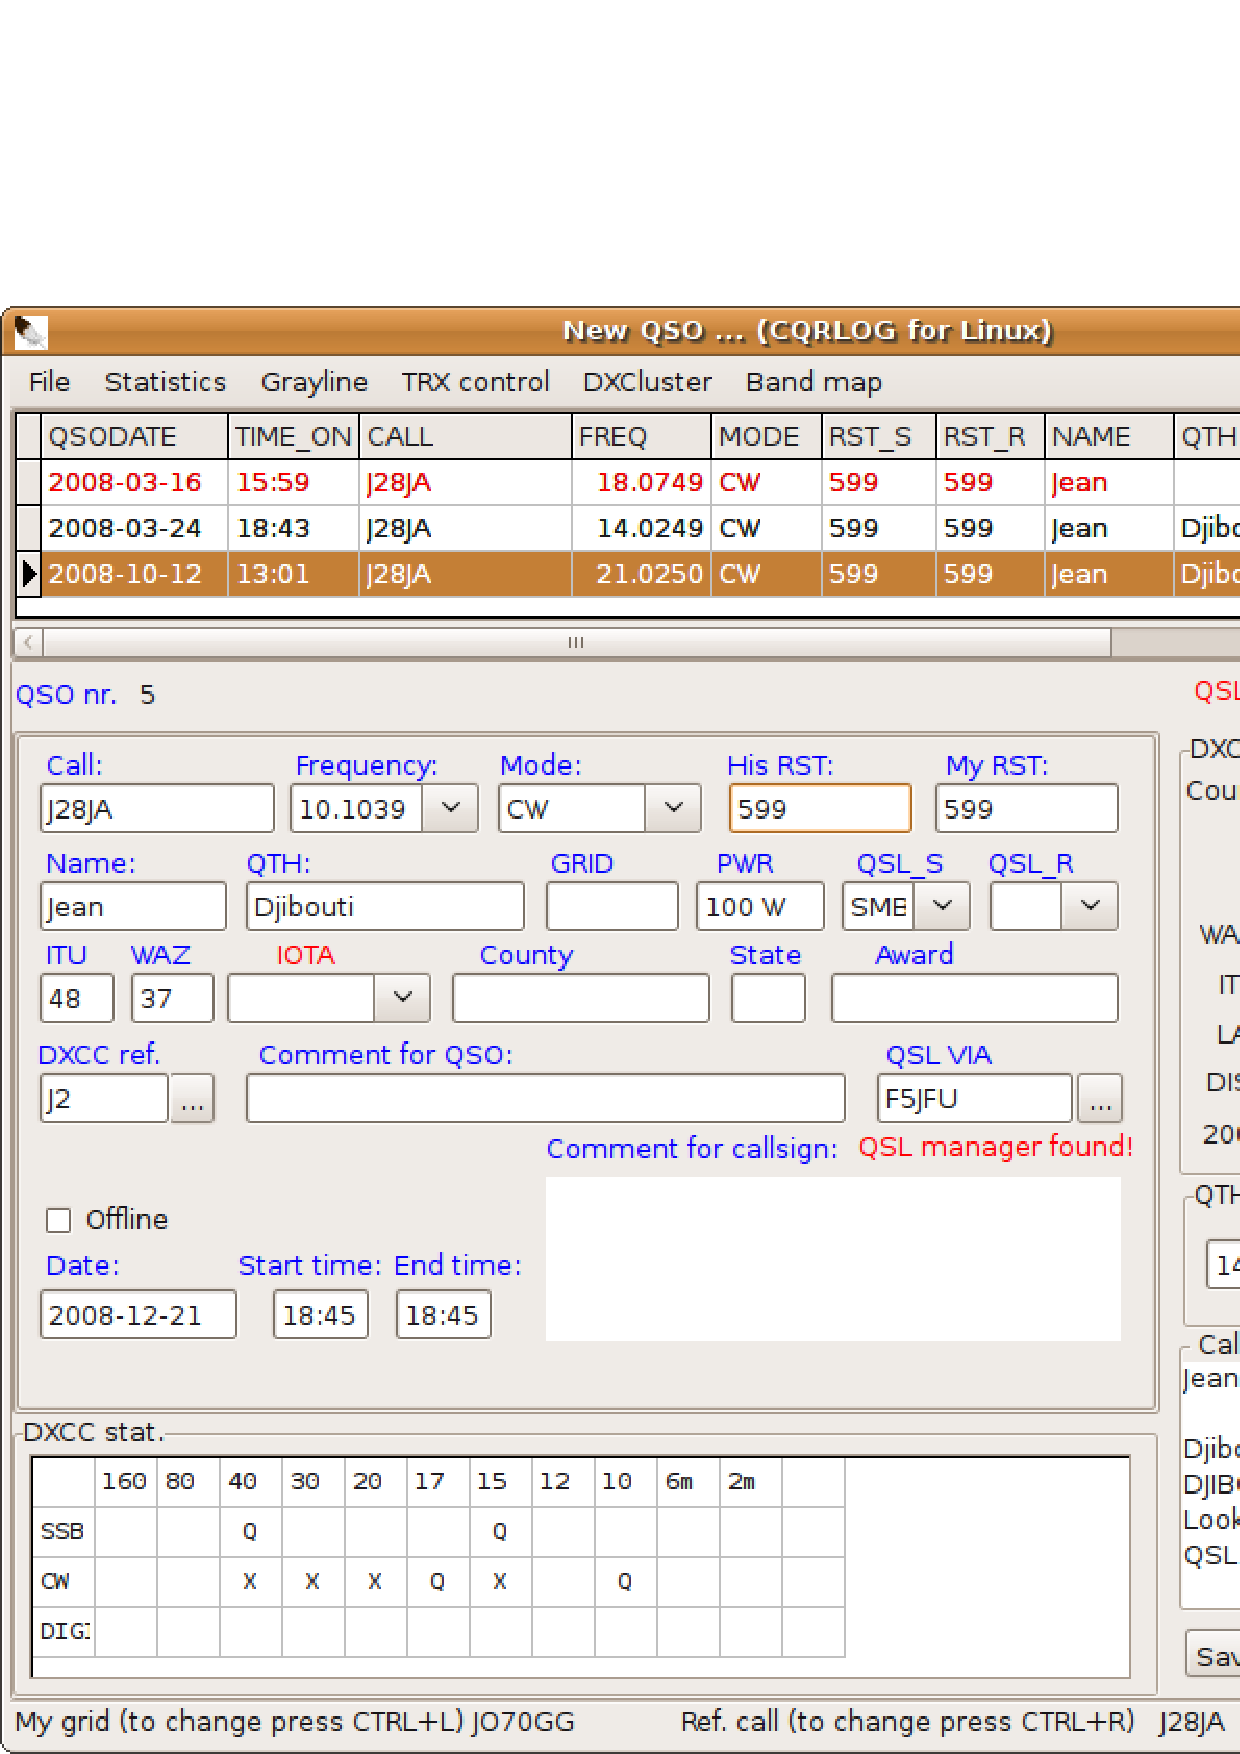
\includegraphics[trim=0cm 0cm 0cm 0cm, scale=0.5]{fig/cqrlog}
\caption{Uživatelské rozhraní CQRLOG.}
\label{fig:cqrlog}
\end{figure}

Jak lze vidět na obrázku \ref{fig:cqrlog}, je jeho uživatelské rozhraní jednodušší než rozhraní programu Logger32 a je
také více přehledné. Na druhou stranu však chybí podpora rozšíření formou pluginů. K dispozici jsou zdrojové kódy v jazyce
Delphi. Ke kompilaci je potřeba vývojového prostředí Lazarus. %% YARDA (DONE): zmínit že to pro kompilaci potřebuje Lazarus 
Volba tohoto programovacího jazyka a závislosti na prostředí Lazarus
značně ztěžuje (až znemožňuje) distribuční integraci, t.j. tvorbu oficiálních instalačních baličků pro linuxové distribuce.

CQRLOG umožňuje použítí
MySQL databáze, ale návrh aplikace znemožňuje jednoduchou změnu databázové aplikace. Také volba MySQL databáze pro použití 
v desktopové aplikaci může být vnímána jako negativum. Návrh CQRLOGu rovněž nedefinuje rozhraní pro jednoduché přidávání nebo úpravu
záznamů pomocí aplikací třetích stran a není tak jednoduché postavit další aplikaci nad CQRLOGem.

\section{HAM Radio Deluxe}

HAM Radio Delux, jehož uživatelské rozhraní lze vidět na obrázku \ref{fig:ham_radio_deluxe}, je dalším ze zástupců
staničních deníků pro operační systém Windows. Uživatelské rozhraní vypadá na první pohled přívětivě a odladěně.
Problémem však může být množství voleb, ve kterých se uživatel lehce ztratí.

\begin{figure}[h]
\centering
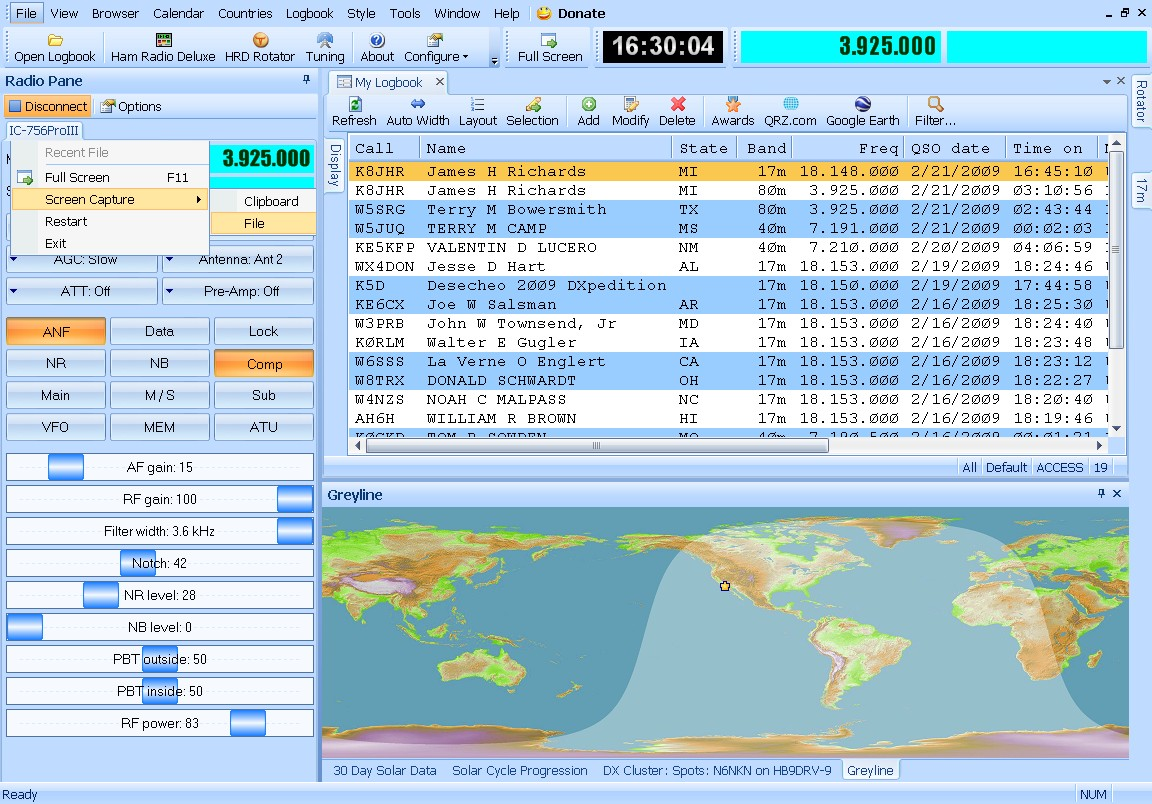
\includegraphics[trim=0cm 0cm 0cm 0cm, scale=0.33]{fig/hrd}
\caption{Uživatelské rozhraní HAM Radio Deluxe.}
\label{fig:ham_radio_deluxe}
\end{figure}

Jedná se o uzavřenou aplikaci, což brání jejímu dalšímu rozšířovaní zájemci z
řad široké veřejnosti. Oproti aplikaci
Logger32 neposkytuje ani API pro tvorbu pluginů. Na druhou stranu obsahuje HAM Radio Deluxe všechny
potřebné nástroje pro provoz staničního deníku. Umožňuje také použití MySQL nebo MSSQL databáze.
Nevýhodou tak zůstává jeho uzavřenost.


\chapter{Návrh}
\label{navrh}

Cílem této kapitoly je návrh aplikace a použitého komunikačního protokolu.

Na základě analýzy z předchozí kapitoly vyplynuly základní požadavky
na výslednou aplikaci.

\begin{itemize}
\item \textbf{Multiplatformnost} - Nutným požadavkem je možnost spuštění
aplikace (nebo přeložení zdrojového kódu) na různých operačních systémech / platformách.
\item \textbf{Architektura klient-server} - Jádro aplikace je tvořeno
serverem. %% YARDA2: je to požadavek, takže by to mělo být dále formulováno podobně
%% jako předchozí požadavek, např. jádro aplikace bude tvořit server, nebo:
%% dalším požadavkem je použití serveru, který umožní vedení deníku více
%% uživatelů.. a podobně dále v této kapitole.
Server umožňuje vedení deníků více uživatelů zároveň a poskytuje rozhraní pro přídavné moduly.
Klientská aplikace se připojí k serveru a prostředníctvím komunikačního protokolu s ním komunikuje.
Díky tomuto rozdělení je možné přidávat záznamy do centrální databáze z více zařízení a pracovat
tak všude se stejnými daty. Využití klient-server architektury je výhodné také pro soutěže, kdy může vyhodnocení
výsledků všech účastníků proběhnout současně na centrálním místě.
\item \textbf{Modulárnost} - Serverová aplikace je založena na modulech. Moduly jsou speciální knihovny rozšiřující funkce
serveru. Moduly umí zpracovávat klientské požadavky a je jim umožněn přístup k deníkům jednotlivých uživatelů. Díky použití modulů
je zajištěna jednoduchá rozšířitelnost aplikace o nové funkce bez nutnosti změny jejího jádra.
\item \textbf{Uložení dat} - Záznamy jednotlivých uživatelů jsou uloženy v databázi SQLite3. Návrh aplikace
však počítá s možností použití různých formátů pro uložení uživatelských dat.
\item \textbf{Oddělení grafického rozhraní od komunikace se serverem} - Klientská aplikace využívající grafického rozhraní
je oddělena od nízkoúrovňové komunikace se serverem díky klientské knihovně. Klientská knihovna obsahuje základní funkce
pro komunikaci se serverem a umožňuje použití libovolného grafického rozhraní bez zbytečné duplikace kódu.
\end{itemize}

Aplikace se tedy skládá z modulárního serveru, klientské knihovny a grafického uživatelského rozhraní.
Toto rozdělení lze vidět i na obrázku \ref{fig:architektura}.
Serverová část funguje nezávisle na klientské části. Obě části však moho bez výrazného dopadu 
na výkonnost běžet lokálně na jednom počítači a výsledná aplikace tak bude použitelná i bez
jakéhokoliv speciálního hardwaru.

V následujících podkapitolách jsou jednotlivé části aplikace stručně popsány.

%% YARDA (DONE): zmínit linux princip KISS (keep it simple and stupid), tedy modulární
%% části, každá dělá svoje, dělá to jednoduše a dobře, pak se to spojí do většího
%% celku. Taky zmínit, že to nemusí běžet rozděleně server klient, ale že to
%% může běžet všchchno lokálně na jednom stroji aniž by tím nějak výrazně utrpěla
%% výkonnost.
\begin{figure}[h]
\centering
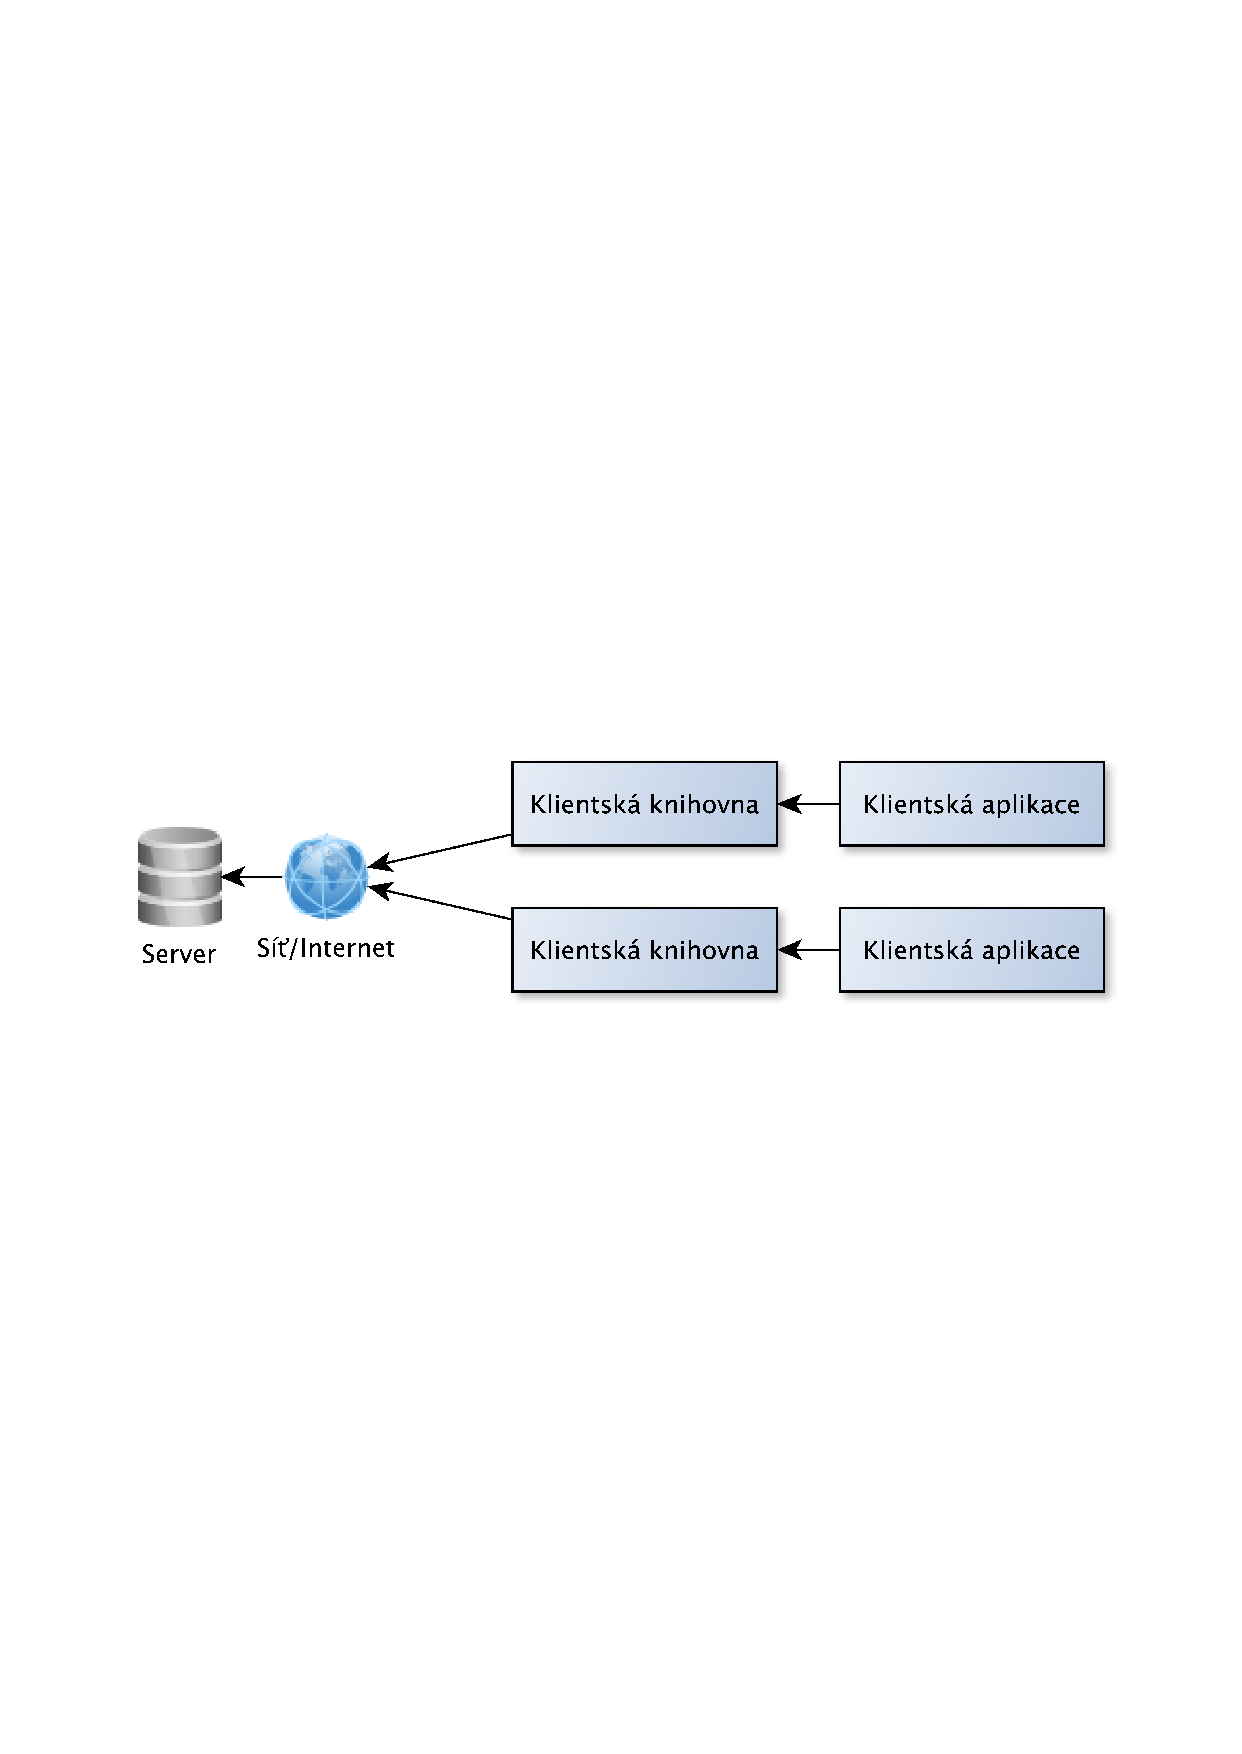
\includegraphics[trim=12cm 12cm 12cm 12cm, scale=0.8]{fig/princip}
\caption{Základní architektura aplikace} %% YARDA: možná raději základní
%% architektura, konzistentnost v pojmech aplikace, program, atd.
%% Ještě bych tam zakreslil ty pluginy.
\label{fig:architektura}
\end{figure}

\newpage
\section{Návrh komunikačního protokolu}
\label{navrh_protokol}

%% DONE: napsat pro lamy proč komunikační protokol, k čemu ho vlastně potřebujeme.
%% a vychválit se, že byl navržen a implementován vlastní protokol, jsou to plus
%% body :)

Komunikační protokol je důležitou součástí síťových aplikací. Určuje, jakým
způsobem spolu komunikuje
klientská a serverová část. Použití příliš jednoduchého a úzce zaměřeného
protokolu by mohlo znemožnit budoucí rozšířitelnost. Naopak použití zbytečně
komplikovaného protokolu by znamenalo složitejší řízení komunikace a náročnější
implementaci.

Pro účel staničního deníku jsem se rozhodl použít vlastní protokol inspirovaný protokolem HTTP \cite{http},
převážně kvůli jeho jednoduchosti a účelnosti z hlediska modularity.

%% YARDA (DONE): taky napsat výhodu prostupnost přes firewally proxy, atp.
Jednotlivé moduly serveru mají své vlastní URI a klientské požadavky jsou pak směrovány podle URI na konkrétní modul,
který generuje odpověď pro klienta. Komunikace tedy probíhá v režimu požadavek-odpověď.

Navržený protokol je zpětně kompatibilní s protokolem HTTP. Díky této kompatibilitě
je dále možné serverovou aplikaci jednoduše napojit na ověřené technologie postavené na bázi HTTP jako je například
AJAX \cite{ajax}. Další výhodou tohoto protokolu je jeho dobrá prostupnost přes
existující HTTP proxy a minimální omezení existujícími firewally.


Přenášená užitečná data jsou ve formátu CSV \cite{csv}, kde první řádek reprezentuje hlavičku dat. Standardní názvy
sloupců ve hlavičce protokolu jsou: %% YARDA2: opět, pokud je kapitola nadepsaná
%% návrh, bylo by dobré psát např: názvy sloupců .. byly zvoleny následovně.. a
%% obdobně dále
\begin{itemize}
\item \textbf{id} - ID záznamu v logu. Koresponduje s ID v databázi a slouží jako klíč pro vybrání konkrétního řádku.
\item \textbf{user\_id} - ID uživatele, jemuž záznam v logu patří.
\item \textbf{qsodate} - Datum záznamu ve formátu unixového timestampu.
\item \textbf{callsign} - Volací značka (například OK2JRQ).
\item \textbf{mode} - Druh provozu. %% YARDA (DONE): příklad
\item \textbf{qth} - QTH lokátor.
\item \textbf{name} - Jméno operátora.
\item \textbf{latitude} - Zeměpisná šířka.
\item \textbf{longitude} - Zeměpisná délka.
\item \textbf{county} - Okres.
\item \textbf{continent} - Zkratka kontinentu.
\item \textbf{cq} - CQ zóna.
\item \textbf{itu} - ITU zóna.
\item \textbf{rst\_tx} - Odeslaný report v systému RST.
\item \textbf{rst\_rx} - Přijatý report v systému RST.
\item \textbf{qsl} - Příznak žádosti o QSL lístek. Pokud je tento příznak nastaven, ví operátor, že si chce
s protistranou vyměnit QSL lístky. To umožňuje případné automatické generování QSL lístků na základě informací
uložených v databázi.
\item \textbf{qsl\_sent} - Příznak poslání QSL lístku. Pokud byly QSL lístky vygenerovány a odeslány, je tento
příznak nastaven.
\item \textbf{qsl\_received} - Příznak přijetí QSL lístku. Tento příznak je nastaven v případě, kdy operátor
obdržel QSL lístek od radioamatéra, se kterým bylo spojení navázáno.
\item \textbf{comments} - Komentáře.
\end{itemize}

Jednotlivé moduly serveru však mohou použít i své vlastní názvy sloupců pro položky, které nejsou v tomto seznamu.

\subsection{Požadavky na komunikační protokol}
%% YARDA (DONE): specifikoval bych výčtem, co všechno ten protokol musí umět a poskytovat,
%% např. přihlášení uživatele a jednotlivé příklady bych přesunul do kapitoly
%% implementace.

V této podkapitole jsou uvedeny případy použití (use cases), které vyplynuly z
analýzy funkce existujících deníků. Tyto případy musí
navrhovaný protokol obsloužit. Pro uvedené případy použití
budou implementovány samostatné moduly (viz podkapitola \ref{navrh_moduly}).

\begin{itemize}
\item Registrace uživatele.
\item Přihlásení uživatele - Přihlášení metodou Digest Access Authentication definovanou v
RFC 2617 \cite{rfc2617}. 
Díky tomu se heslo neposílá %% YARDA2: opět návrh, tedy: .. heslo se numusí
%% posílat po síti 
při přihlášení po síti a na straně serveru je možné ukládat
pouze jeho otisk vytvořený funkcí MD5 \cite{md5}. To znemožňuje zjištění hesla odposlechem nebo jeho odcizení ze
serveru.
\item Vyžádání kompletního deníku nebo jeho částí.
\item Vložení nového záznamu, jeho následná editace a případné odstranění.
\item Zjištění detailních informací o majiteli volacího znaku.
\item Ovládání radiostanice - změna a zjištění frekvence.
\item Získání dat ze služby DXCluster.
\end{itemize}

\subsection{Ukázky použití protokolu}
%% YARDA2: toto spíše do implementace

\subsubsection{Vyžádání logu}

Tento příklad ukazuje použití protokolu pro získání všech záznamů z logu.

Dotaz na modul poskytující URI "/logbook":
\begin{verbatim}
GET /logbook HTTP/1.1


\end{verbatim}
Odpověď serveru:
\begin{verbatim}
HTTP/1.1 200 OK
Content-Type: text/hamlog
Content-Length: 74

id;user_id;callsign;date;qth;loc
1;1;TEST;2011;qt;
2;1;LKS;2011;;location
\end{verbatim}

\subsubsection{Ukázka přihlášení uživatele}

Dotaz na modul poskytující URI "/login":
\begin{verbatim}
GET /login HTTP/1.1

\end{verbatim}

Odpověď serveru vybízí uživatele k přihlášení podle RFC 2617 \cite{rfc2617}:
\begin{verbatim}
HTTP/1.0 401 Unauthorized
Content-Type: text/html
Content-Length: 14
WWW-Authenticate: Digest realm="realm@hamlog",qop="auth,auth-int",nonce="dcd98b7102dd2f0e8b11d0f600bfb0c093",opaque="5ccc069c403ebaf9f0171e9517f40e41"

Authentication
\end{verbatim}

Klient se přihlásí s použitím správného jména a hesla, které je však přenášena
zahashované:
\begin{verbatim}
GET /login HTTP/1.1
Authorization: Digest username="ok2jrq",realm="realm@hamlog",nonce="dcd98b7102dd2f0e8b11d0f600bfb0c093",uri="/login",qop=auth,response="d197141dc972c02d71e6a73b3396ed53",opaque="5ccc069c403ebaf9f0171e9517f40e41")

\end{verbatim}

Server informuje klienta o úspěšném přihlášení:
\begin{verbatim}
HTTP/1.1 200 OK
Content-Type: text/html
Content-Length: 10

Authorized
\end{verbatim}

\section{Návrh serveru}
\label{navrh_server}

Server je aplikace bez uživatelského rozhraní %% YARDA (DONE): místo konzolová aplikace raději aplikace
%% bez uživatelského rozhraní 
zpracovávající klientské požadavky. Administrátor může server konfigurovat konfiguračním souborem
%% YARDA2: opět návrh tedy např.: požadavkem je možnost konfigurace pomocí
%% souborů v INI  formátu
v INI formátu. %% YARDA (DONE): popsat co to je, nebo link 
Jedná se o jednoduchý formát umožňující rozdělit konfiguraci do kategorií
a v každé definovat dvojice klíč=hodnota sloužící ke konfiguraci. Použití INI formátu lze vidět na následující
ukázce konfigurace serveru:

\begin{verbatim}
[server]
hostname = 127.0.0.1
port = 8080

[database]
type = sqlite3
database = test.sql
\end{verbatim}
 
Server je schopen obsluhovat více uživatelů současně.
Uživatelé se k serveru přihlašují pomocí jména a hesla. Noví uživatelé se musí nejprve registrovat.

Návrh serveru počítá s použitím libovolné databáze pro uchování perzistentních dat. V rámci této bakalářské práce jsem se 
rozhodl použít databázi SQLite3.

Server je modulární a veškeré služby, které uživateli poskytuje, jsou součástí modulů. Server samotný pouze spravuje
připojené uživatele a deleguje požadavky na jednotlivé moduly.

\subsection{Moduly}
\label{navrh_moduly}

Moduly umožňují dynamicky rozšiřovat funkčnost serveru. Každý nový požadavek, který server od klienta přijme je
předán příslušnému modulu na základě URI (viz obrázek \ref{fig:navrh_moduly}).
Modul jej zpracuje a odešle klientovi zpět odpověď. Klient si může
od serveru vyžádat seznam všech modulů pomocí požadavku na speciální URI "/modules".

Modulům je také umožněno přistupovat k databázi záznamů všech uživatelů a provádět nad ní dotazy. Tato problematika je více
rozebrána v následující podkapitole \ref{navrh_databaze}.

\begin{figure}[h]
\centering
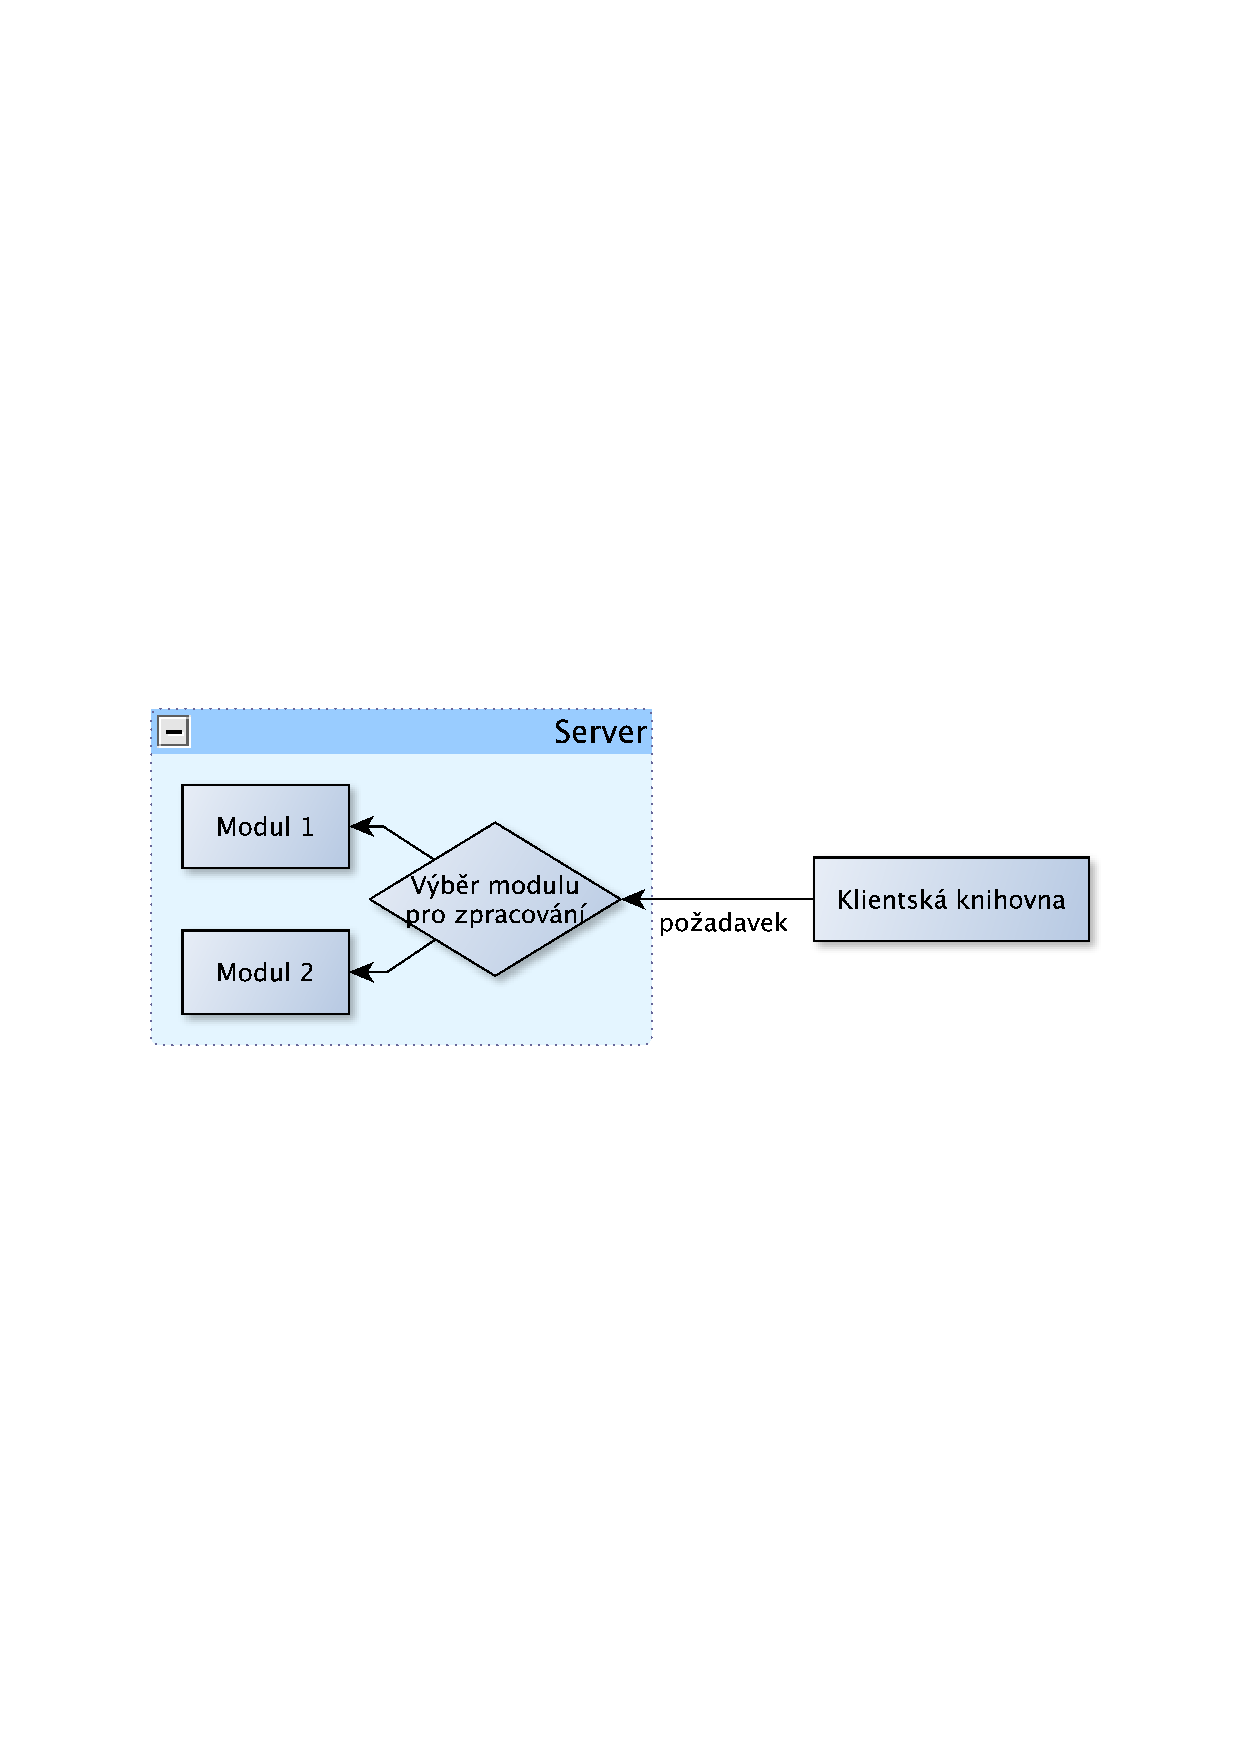
\includegraphics[trim=11cm 11cm 11cm 11cm, scale=0.7]{fig/navrh_moduly}
\caption{Návrh využití modulů.}
\label{fig:navrh_moduly}
\end{figure}

Jednotlivé moduly serveru jsou navrženy jako dynamické knihovny.
Při spuštění serveru jsou nahrány všechny moduly z adresáře nastavitelného pomocí konfiguračního souboru.

Každý modul obsahuje následující informace:

\begin{itemize}
\item \textbf{URI} - URI modulu, na kterém daný modul pracuje. Každý modul serveru musí mít své jedinečné URI.
\item \textbf{Typ} - Typ modulu. Všechny moduly daného typu poskytují stejné komunikační rozhraní. To umožňuje klientské knihovně
komunikovat i s pro ni neznámými moduly pouze na základě znalosti jejich typu.
\item \textbf{Popis} - Krátký text popisující funkci modulu. V grafickém rozhraní je tento text zobrazen v seznamu modulů.
\end{itemize}

V rámci této bakalářské práce byly implementovány moduly následujících typů (lze
však rozšířit):

\begin{itemize}
\item \textbf{CALLINFO} - Moduly tohoto typu poskytují rozličné informace (například polohu nebo jméno operátora)
na základě volací značky. Data jsou získávána z veřejně dostupných služeb, nebo z databáze uložené na serveru.
\item \textbf{DXCLUSTER} - Moduly typu DXCLUSTER poskytují informace (například frekvenci a polohu) o stanicích,
které aktuálně vysílají.
\end{itemize}

\subsubsection{Rozhraní modulů typu CALLINFO}

S moduly typu CALLINFO lze komunikovat následujícími způsoby:

\begin{itemize}
\item \textbf{Požadavek typu POST na URI "/modul"} - %% YARDA:  link co to je
%% POST
Jako data je v požadavku zaslána volací značka operátora. Odpověď obsahuje
veškeré zjistitelné informace o volací značce ve formátu CSV definovaném v podkapitole \ref{navrh_protokol}.
\item \textbf{Požadavek typu GET na URI "/modul/username"} - %% YARDA: link co
%% to je GET
Pokud modul vyžaduje registraci uživatelského jména a hesla pro
přístup k databázi volacích značek (například v případě, že modul přistupuje ke službě, která je jen pro registrované), musí modul
implementovat zpracování tohoto URI a vrátit aktuálně registrované uživatelské jméno nebo prázdný řetězec. Klient pak může tohoto
chování využít pro zjištení, jestli je potřeba být pro použití modulu registrován.
\item \textbf{Požadavek na URI "/modul/register"} - Slouží k registraci uživatelského jména a hesla pro použití modulu.
Jméno a heslo jsou předány v hlavičce paketu pod klíči "username" a "password".
\end{itemize}

\subsubsection{Rozhraní modulů typu DXCLUSTER}

Moduly typu DXCLUSTER poskytují následující funkce:

\begin{itemize}
\item \textbf{Požadavek typu GET na URI "/modul"} - Modul vrátí seznam nově vysílajících stanic od posledního dotazu. Klient se tak
musí opakovaně ptát, aby získal nové vysílající stanice.
\item \textbf{Požadavek typu GET na URI "/modul/username"} - Význam je stejný jako u modulu typu CALLINFO.
\item \textbf{Požadavek na URI "/modul/register"} - Význam je stejný jako u modulu typu CALLINFO.
\end{itemize}

\subsection{Databáze}
\label{navrh_databaze}

Součástí serveru je rozhraní pro přístup k databázi. Veškerá data všech
uživatelů jsou uložena v této databázi.
Návrh serveru počítá s využitím databáze jakéhokoliv typu (SQLite3, MySQL, PostgreSQL, \dots). Jednotlivé moduly
umí prostřednictvím databázového rozhraní s databází pracovat a spouštět nad ní prakticky libovolné dotazy.

Na obrázku \ref{fig:databaze} je zobrazeno obecné schéma databáze použité pro uložení všech potřebných informací. Tabulky
z tohoto obrázku jsou pak dále stručně popsány.

\begin{figure}[h]
\centering
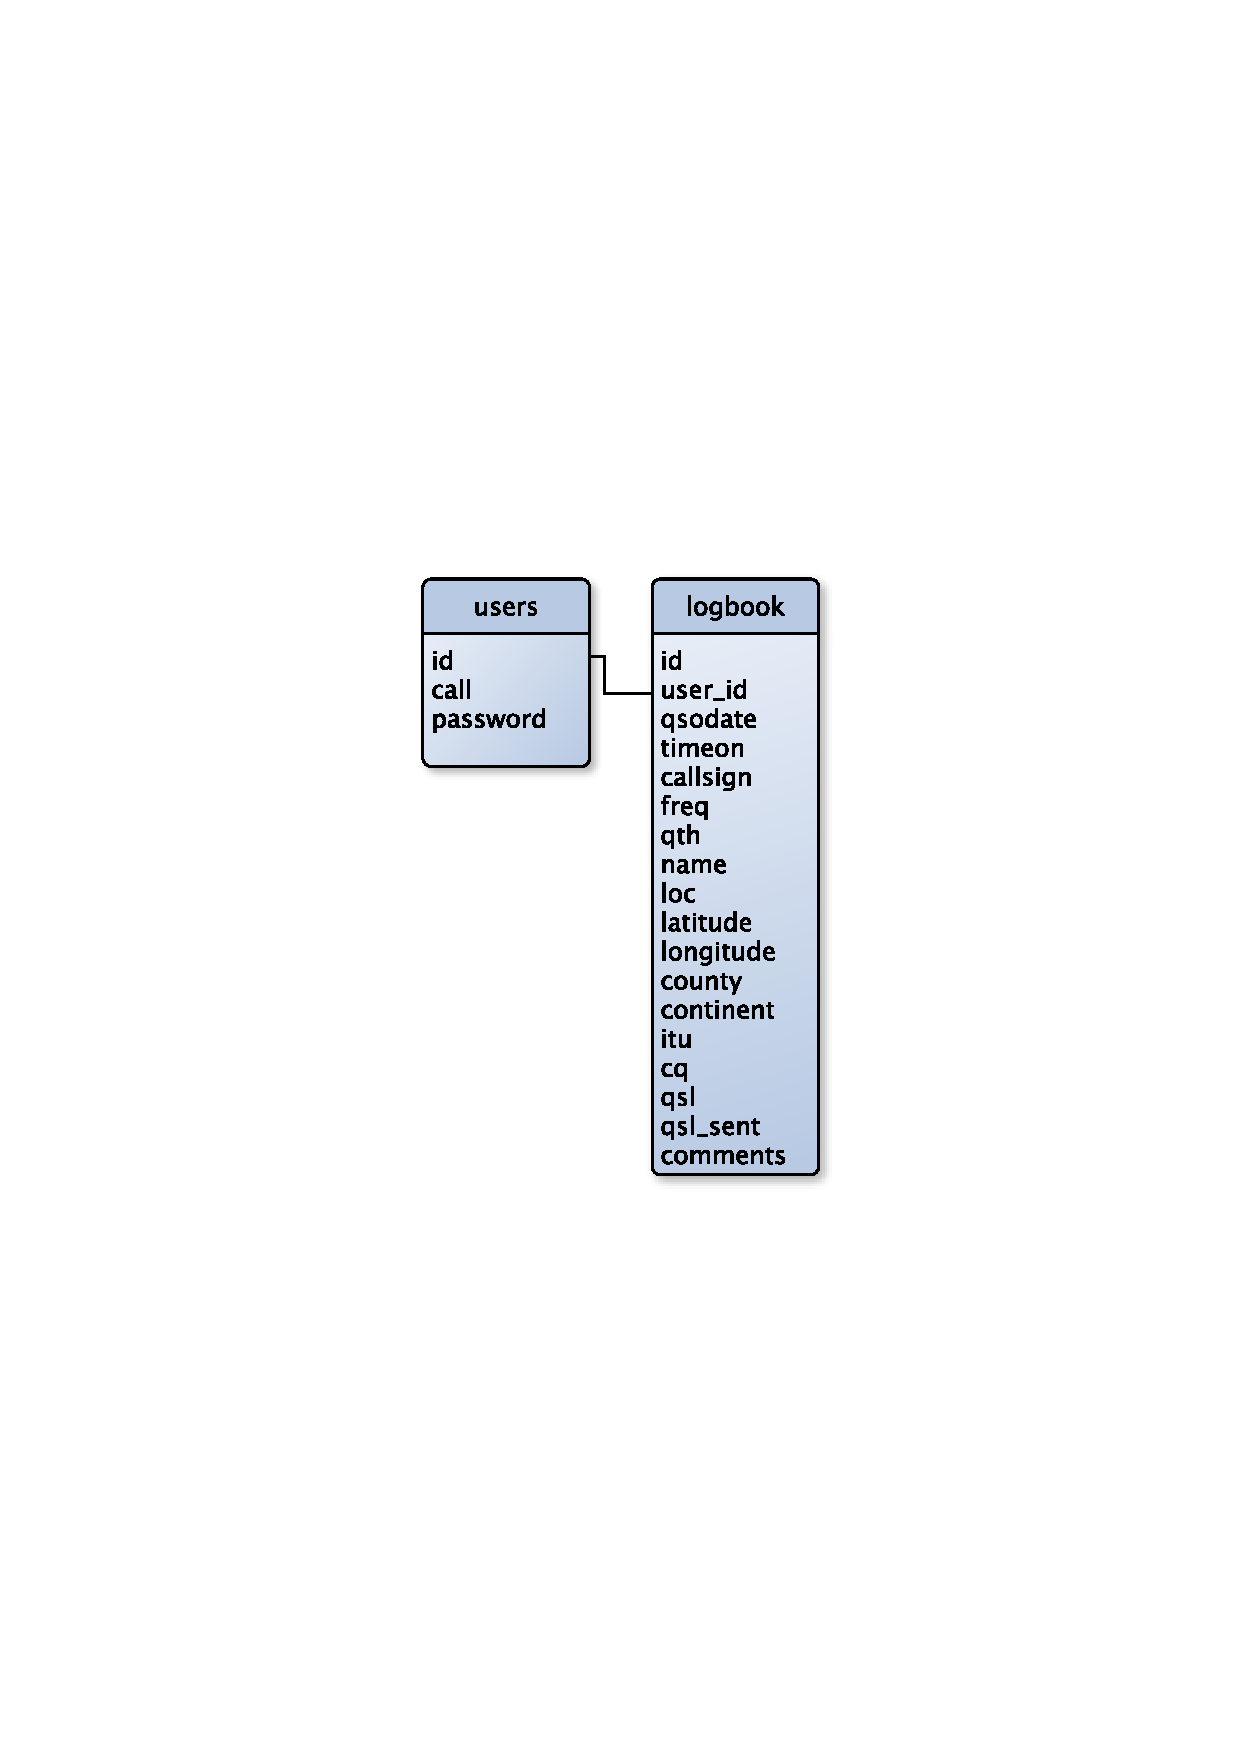
\includegraphics[trim=9cm 9cm 9cm 9cm, scale=0.7]{fig/navrh_databaze}
\caption{Návrh databáze.}
\label{fig:databaze}
\end{figure}

\subsubsection{Tabulka users}

Tabulka users obsahuje informace potřebné pro přihlášení uživatele (deník může
používat více uživatelů). Každý uživatel zde má uloženo ID, volací značku a
heslo.

\subsubsection{Tabulka logbook}

V tabulce logbook jsou uloženy deníky všech uživatelů. Obsahuje následující sloupce:

\begin{itemize}
\item \textbf{id} - ID záznamu.
\item \textbf{user\_id} - ID uživatele, jemuž záznam patří.
\item \textbf{qsodate} - Datum záznamu ve formátu Unix timestamp.
\item \textbf{callsign} - Volací značka (například OK2JRQ).
\item \textbf{mode} - Druh provozu. %% YARDA (DONE): příklad
\item \textbf{qth} - QTH lokátor (Maidenhead Locator).
\item \textbf{name} - Jméno operátora.
\item \textbf{latitude} - Zeměpisná šířka.
\item \textbf{longitude} - Zeměpisná délka.
\item \textbf{county} - Okres.
\item \textbf{continent} - Zkratka kontinentu.
\item \textbf{cq} - CQ zóna.
\item \textbf{itu} - ITU zóna.
\item \textbf{rst\_tx} - Odeslaný report v systému RST.
\item \textbf{rst\_rx} - Přijatý report v systému RST.
\item \textbf{qsl} - Příznak žádosti o QSL lístek. Pokud je tento příznak nastaven, ví operátor, že si chce
s protistranou vyměnit QSL lístky. To umožňuje případné automatické generování QSL lístků na základě informací
uložených v databázi.
\item \textbf{qsl\_sent} - Příznak poslání QSL lístku. Pokud byly QSL lístky vygenerovány a odeslány, je tento
příznak nastaven.
\item \textbf{qsl\_received} - Příznak přijetí QSL lístku. Tento příznak je nastaven v případě, kdy operátor
obdržel QSL lístek od radioamatéra, se kterým bylo spojení navázáno.
\item \textbf{comments} - Komentáře.
\end{itemize}

\section{Klientská knihovna}
\label{navrh_knihovna}

Klientská knihovna poskytuje grafickému rozhraní jednotné API pro přístup k
serveru. To zamezuje duplikaci kódu při případné implementaci více
různých grafických rozhraní využívajících funkce serveru.

Klientská knihovna má minimální závislosti a je multiplatformní. Pomocí komunikačního protokolu
komunikuje se serverem, zpracovává příchozí data a předává je klientovi.

Knihovna je navržena tak, aby mohla spolupracovat s jakýmkoliv grafickým
rozhraním (například Qt, GTK, wxWidgets, ncurses, \dots). %% YARDA (DONE): blíže specifikovat, co se myslí, QT, GTK?

Základní funkce klientské knihovny jsou:

\begin{itemize}
\item Připojení k serveru, registrace a přihlášení uživatele.
\item Generování požadavků pro server a jejich předání serveru.
\item Zpracování odpovědí serveru a předání zpracovaných dat klientské knihovně.
\end{itemize}

\section{Klient}
\label{navrh_klient}

Klient umožňuje uživateli připojení k serveru, prezentaci aktuálních dat a
jejich změny. Pro komunikaci
se serverem klient využívá klientskou knihovnu. Pro komunikaci s uživatelem pak klient využívá grafického rozhraní.
Po startu klienta je uživatel vyzván k přihlášení se k serveru. Uživateli je rovněž nabídnuta možnost registrace
nového účtu.

Po přihlášení zobrazí klientská aplikace veškeré záznamy v deníku a umožní jejich editaci. Klientská aplikace také zobrazuje
aktuální vysílání získané ze služby DXCluster. Stanice, které aktuálně vysílají jsou zobrazeny graficky na modelu 
zeměkoule.

Po vybrání stanice je zobrazen dialog pro přidání nového záznamu s předvolenými hodnotami získanými ze služby DXCluster. Automaticky
je také přeladěno rádio na danou frekvenci.

V okně pro nový záznam je uživateli zobrazena historie všech spojení s daným operátorem.
Po potvrzení dialogu je nový záznam odeslán na server a uložen do databáze.

Klient také umožňuje zobrazit všechny moduly dostupné na serveru a jejich
textový popis.


\chapter{Implementace}
\label{implementace}

V této kapitole je popsána implementace serverové aplikace, klientské aplikace a klientské knihovny.

\section{Serverová aplikace}
\label{implementace_server}

Server byl implementován v jazyce C++ umožňujícím lepší dekompozici aplikace a
použití objektově orientovaného přístupu. Byla rovněž
použita knihovna Boost, která poskytuje základní metody pro asynchronní síťovou komunikaci a nabízí programátorské prostředky
nad rámec standardní STL knihovny.

Pro implementaci modulu QRZ bylo potřeba použít knihovnu pro zpracování XML. K
tomuto účelu byla použita knihovna TinyXML.

Dále budou stručně popsány nejdůležitejší třídy serveru.

\subsubsection{Třída Server}

Třída Server je základní třídou serveru. Vytváří soket, na kterém server přijímá připojení z klientské knihovny. Jakmile je 
akceptováno nové připojení, je vytvořena instance třídy Session, která dále
zpracovává všechny požadavky klienta.

\subsubsection{Třída Session}

Tato třída reprezentuje sezení jednoho uživatele. Při obdržení nových dat od klienta jsou tato předána instanci třídy
RequestParser, která slouží k jejich rozparsování. Pokud byla obdržena kompletní zpráva, je předána instanci třídy 
ModuleManager metodou handleRequest, která pak řídí její další zpracování. Výsledná odpověď je pak instancí třídy Session poslána
zpět klientovi.

\subsubsection{Třída RequestParser}

Třída RequestParser reprezentuje konečný automat pro parsování zpráv podle specifikace komunikačního protokolu.
Metoda parse zpracovává přijatá data, parsuje je, a výsledek uchovává v instanci třídy Request. Pokud dojde během parsování
k chybě, vrací funkce parse hodnotu false a uživatel, jehož klient poslal
neplatná data, je odpojen.

\subsection{Databázové rozhraní}
\label{implementace_db}

Návrh a implementace serveru umožňuje použití libovolného databázového rozhraní.
V rámci bakalářské práce však byla implementována 
pouze podpora pro databázi SQLite3 (lze však snadno rozšířit). Třída implementující konkrétní databázové rozhraní musí dědit třídu StorageBackend a implementovat
její čistě virtuální metody \cite{oop}. Vztah jednotlivých tříd implementujících a využívajících databázové rozhraní lze vidět
na obrázku \ref{fig:imp_databaze}.

\begin{figure}[h]
\centering
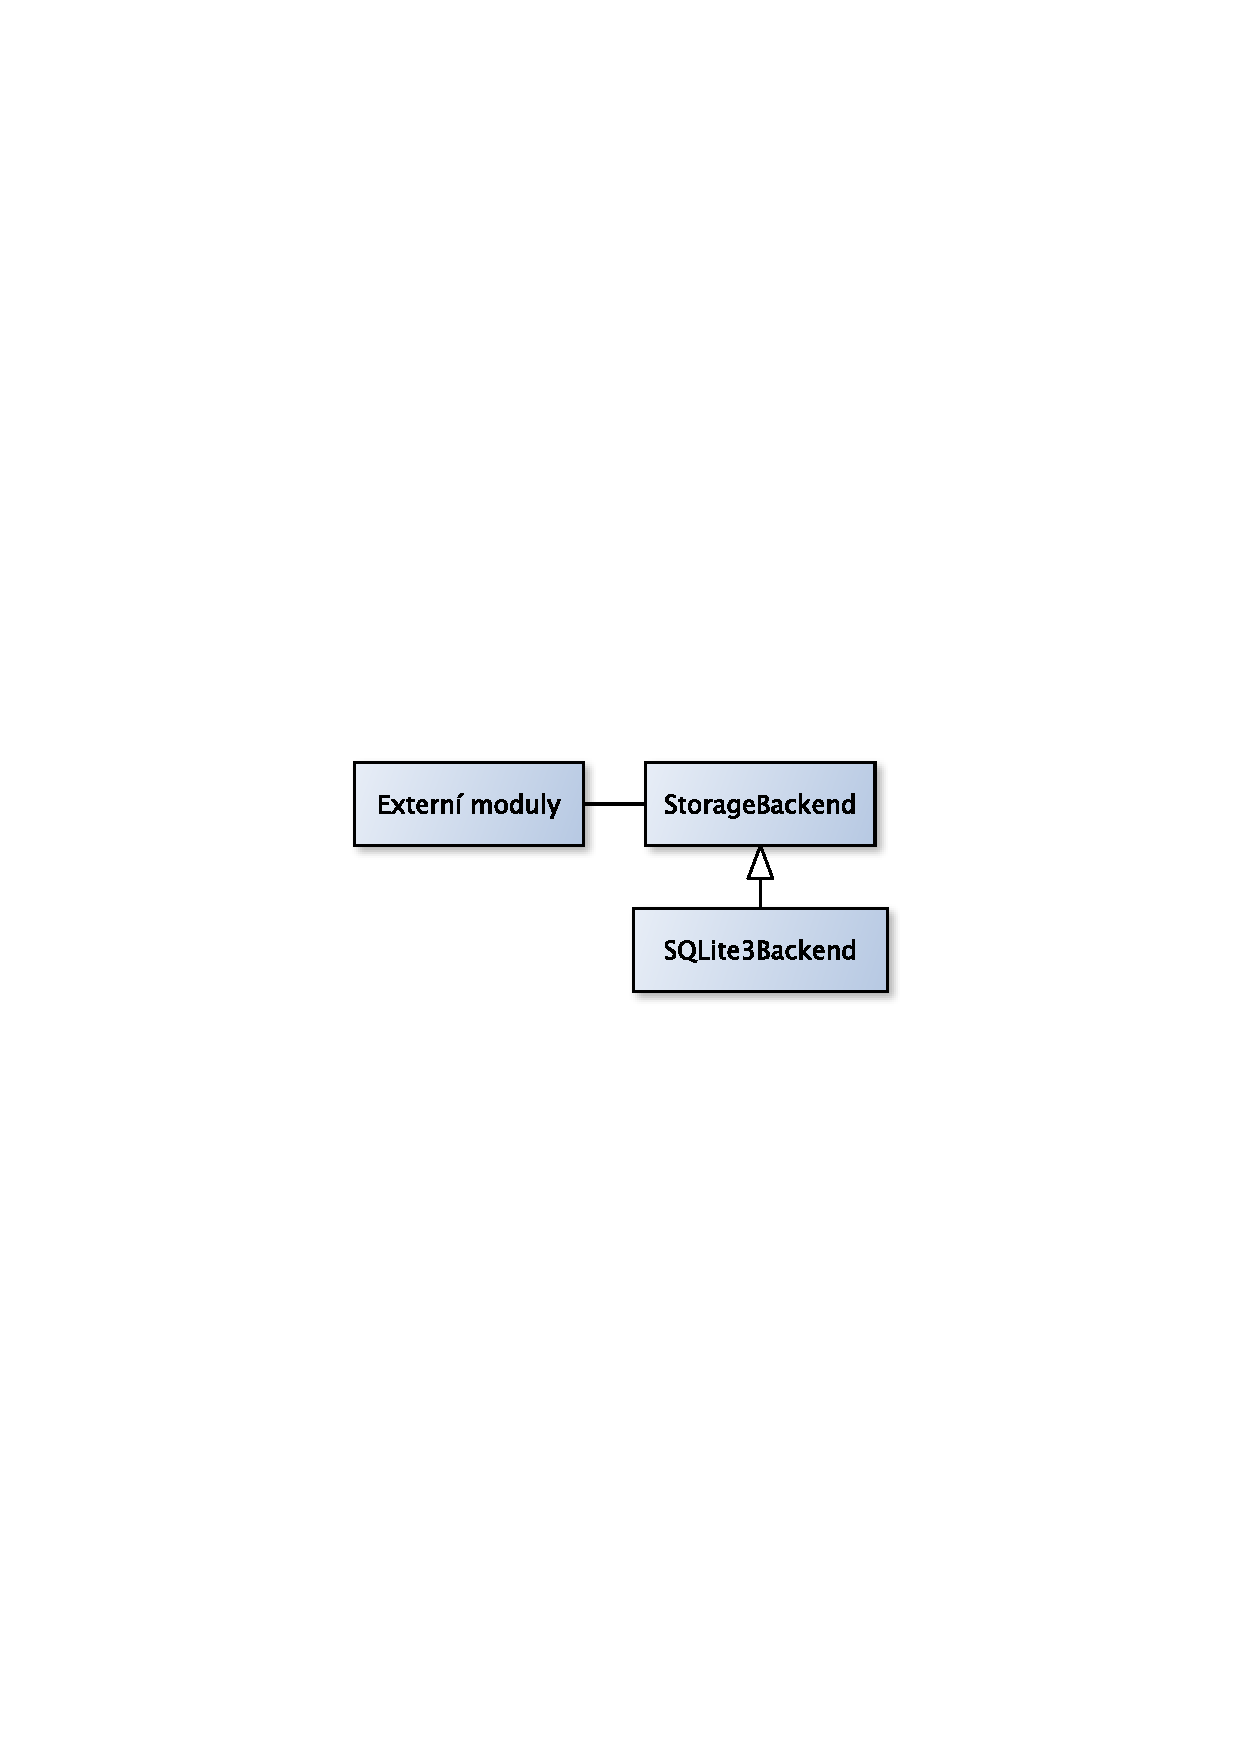
\includegraphics[trim=12cm 12cm 12cm 12cm, scale=0.7]{fig/imp_databaze}
\caption{Diagram databázového rozhraní.}
\label{fig:imp_databaze}
\end{figure}

\subsubsection{Třída StorageBackend}

Třída StorageBackend je základní abstraktní třídou pro implementaci jakéhokoliv databázového rozhraní.
Je u ní použit návrhový vzor Singleton. %% YARDA (DONE): více rozvést, nebo link do literatury
Jedná se o způsob návrhu třídy, který počítá s jedinou instancí dané třídy v rámci celé aplikace.
Tato instance je pak přístupná ze všech částí aplikace. Typicky má třída používající návrhový
vzor Singleton privátní konstruktor a statickou přístupovou metodu vracející instanci této třídy.

Smyslem třídy StorageBackend je poskytnout rozhraní pro získávání dat z databázového rozhraní bez znalosti
typu databáze. Názvy metod a podtříd jsou inspirovány terminologií známou z
oblasti SQL databází, %% YARDA: opět by se hodil link
 ale prakticky
lze pomocí třídy StorageBackend implementovat rozhraní pro přístup k jakémukoliv typu databáze.

Třída StorageBackend obsahuje základní podtřídy pro definici dotazů typu SELECT (používaný pro získání
dat z databáze), INSERT (používaný pro vložení nových dat do databáza), UPDATE (sloužící k aktualizaci
již uložených dat v databázi) a CREATE (umožňující vytvoření nové tabulky) známých z jazyka SQL:

\begin{itemize}
\item StorageBackend::Column - Slouží pro definici sloupce při vytváření nové tabulky metodou StorageBackend::createTable().
Obsahuje veškeré informace o sloupci tabulky:
\begin{itemize}
\item Jméno - Jednoznačně pojmenovává sloupec. Jméno sloupce je pak použito pro výběr konkrétních sloupců v dalších typech
dotazů.
\item Typ - Určuje typ sloupce. V současné implementaci existují tyto 4 typy: celé číslo, desetinné číslo, řetězec, datum a čas.
\item Velikost - Používá se pouze pro sloupce typu řetězec. Udává maximální velikost řetezce uloženého v tomto sloupci.
\item Příznak NOT NULL - Pokud je nastaven, musí být při přidání nebo editaci řádku v tabulce definována hodnota tohoto sloupce.
\item Příznak UNIQUE - Pokud je nastaven, musí být při přidání nebo editaci řádku tabulky hodnota tohoto sloupce jedinečná v rámci
celého sloupce dané tabulky.
\item Příznak PRIMARY KEY - Pokud je nastaven, je tento sloupec primárním klíčem tabulky.
\end{itemize}
\item StorageBackend::Select - Zapouzdřuje data potřebná pro provedení výběru dat z databáze nebo odstranění dat z databáze.
Obsahuje jméno tabulky,
ze které se výběr provádí, a ukazatel na dvourozměrné pole, do kterého se uloží případné
výsledky. Dále třída StorageBackend::Select umožňuje
definovat omezení výběru (v SQL jazyce klíčové slovo WHERE) a umožňuje výběr konkrétních sloupců, které vrátí ve výsledku.
Instance této třídy je předána metodě StorageBackend::select() nebo StorageBackend::remove().
\item StorageBackend::Insert - Obsahuje data pro vložení (v SQL jazyce klíčové
slovo INSERT) nebo aktualizaci (v SQL jazyce klíčové slovo UPDATE)
záznamu v databázi. Obsahuje název tabulky, ve které se budou data měnit, a samotná data ve formě název sloupce - hodnota.
Umožňuje definovat omezení (v SQL jazyce klíčové slovo WHERE) aplikovaná při aktualizaci dat. Instance této třidy je předána metodě
StorageBackend::insert() nebo StorageBackend::update().
\end{itemize}

V závislosti na implementaci metod třídy StorageBackend je pak v některé z
jejich dceřiných tříd provedna konkrétní změna v
databázi. Třída StorageBackend dále umožňuje získání identifikačního čísla naposledy vloženého záznamu metodou lastInsertedID().


\subsubsection{Třída SQLite3Backend}

Tato třída dědí třídu StorageBackend a implementuje její metody pro použití databázového systému SQLite3. V metodách
update(), insert(), select(), createTable() a remove() se na základě předaných
dat vygeneruje dotaz v SQL jazyce, ten se spustí
a je vrácen výsledek.

\subsection{Moduly}
\label{implementace_moduly}

Moduly jsou implementovány jako dynamické knihovny. Každý implementovaný modul dědí třídu Modul (zprostředkovaně například přes třídu RequestResponder)
a implementuje její čistě virtuální
(pure virtual) metody (\cite{oop}). Toto demonstruje obrázek \ref{fig:moduly}. %% YARDA (DONE): hodil by se odkaz na nějakou knihu o OOP 
Veškeré klientské požadavky jsou pak směrovány na konkrétní modul podle URI instancí třídy ModuleManager.

%% YARDA (DONE): každý obrázek musí být odkazován v textu, např. Na obrázku
%% \ref{fig:FigureExample} je zobrazen diagram tříd modulů..

\begin{figure}[h]
\centering
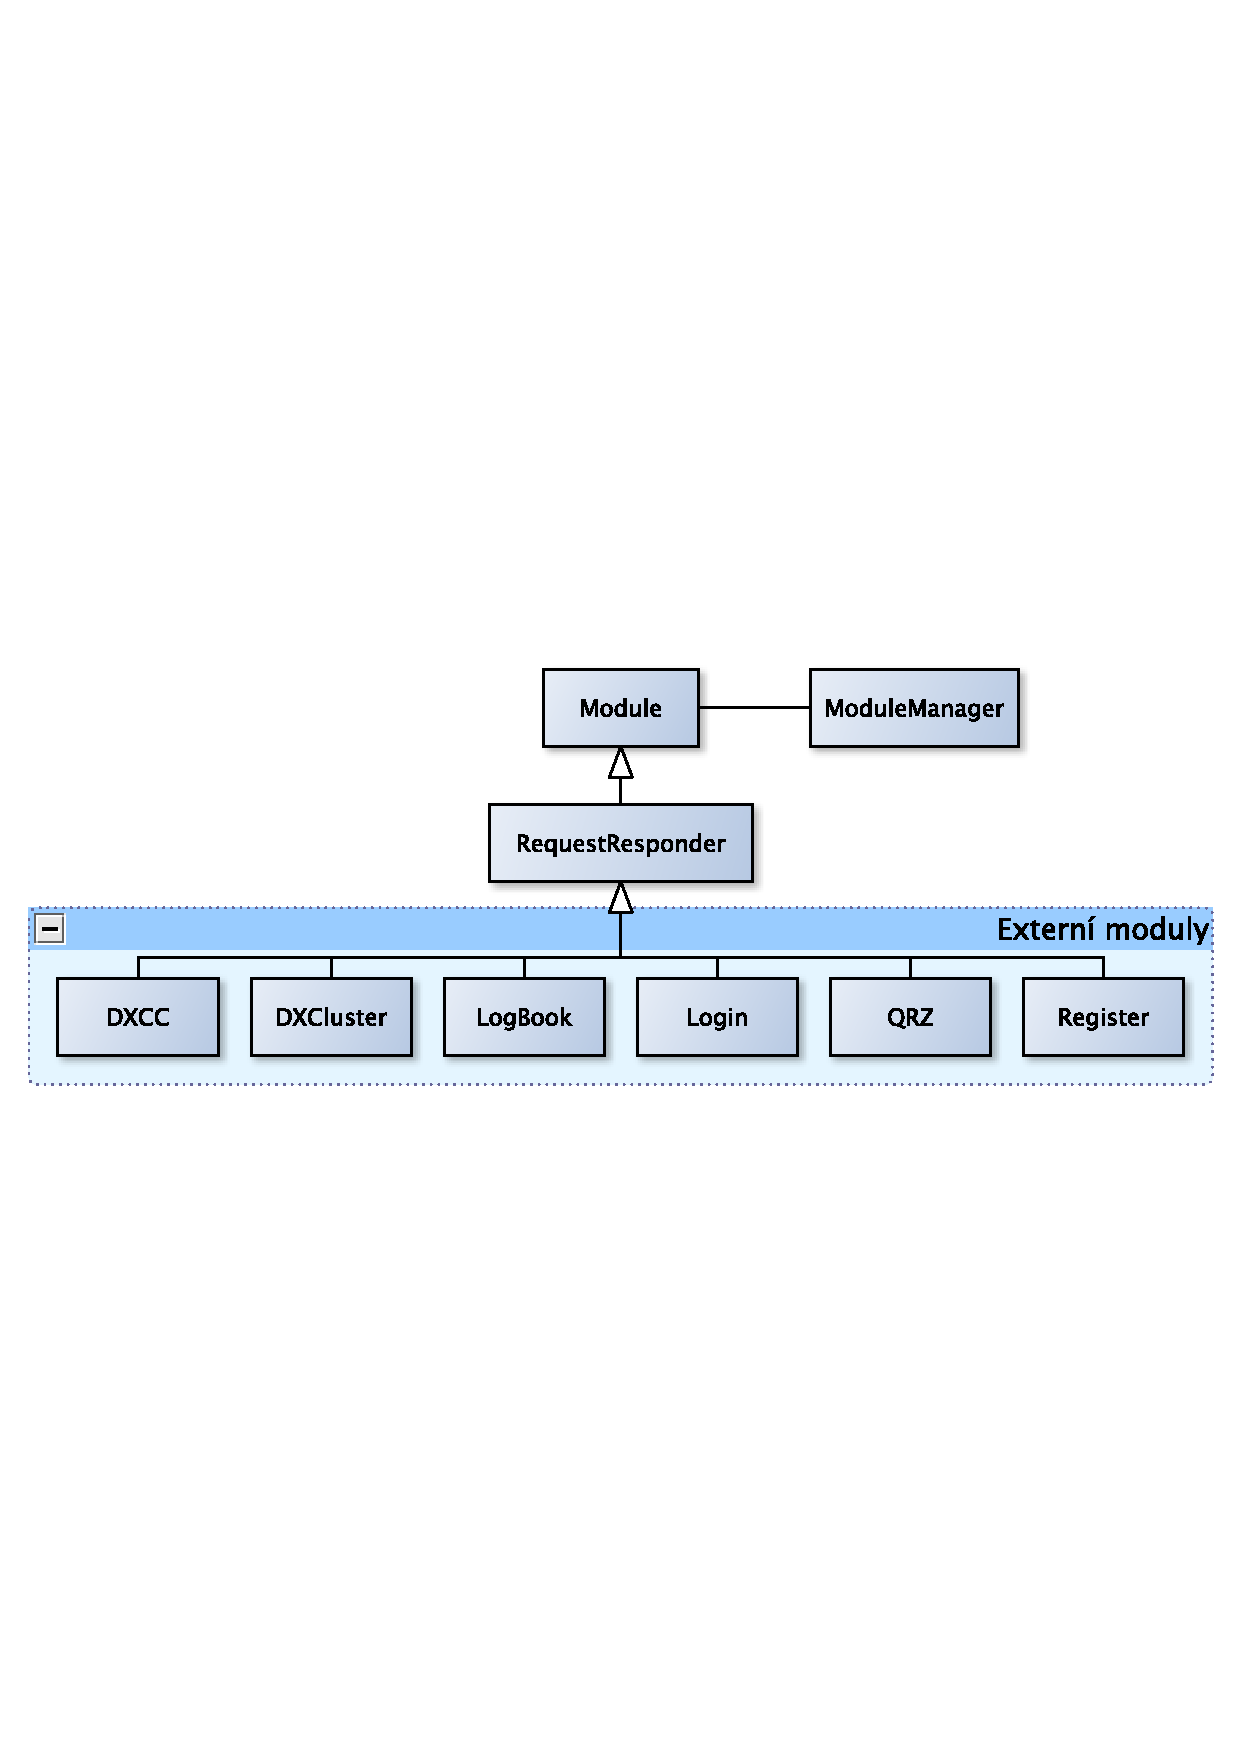
\includegraphics[trim=10cm 10cm 10cm 10cm, scale=0.7]{fig/moduly}
\caption{Diagram tříd modulů.}
\label{fig:moduly}
\end{figure}

\subsubsection{Třída Module}

Třída Module poskytuje základní třídu, kterou musí implementovat každý externí modul. Obsahuje základní informace o modulu 
(jeho jméno, typ a popis).

\subsubsection{Třída RequestResponder}

Tato třída dědí třídu Module a rozšiřuje ji o data a metody specifické pro modul odpovídající na klientské požadavky.
Přiřazuje modulu jeho URI a informaci o tom, jestli musí být uživatel pro jeho použití přihlášen.
Obsahuje také deklaraci metody handleRequest(), která je volána instancí třídy ModuleManager pro každý příchozí požadavek
smeřující na modul.

\subsubsection{Třída ModuleManager}

U třídy ModuleManager je použit návrhový vzor Singleton.
Tato třída zabezpečuje veškerou práci serveru s externími moduly. Pomocí 
metody loadModules lze načíst všechny moduly z adresáře zvoleného v konfiguračním souboru. Veškeré požadavky od klientů
jsou předány instanci této třídy metodou handleRequest, která je pak dále směruje podle URI na konkrétní modul. Třída také
umožňuje poslat seznam všech modulů klientské aplikaci.

\subsection{Implementované moduly} %% YARDA: možná raději implementované moduly - DONE
\label{implementovane_moduly}

V této podkapitole jsou popsány jednotlivé implementované moduly.

\subsubsection{Modul Register}

Modul Register (URI "/register") %% YARDA: 'běžící na' bych odstranil (DONE)
slouží k registraci nových uživatelů. Při svém spuštění vytvoří pomocí
instance třídy StorageBackend tabulku "users". V metodě handleRequest pak přijímá případné požadavky na registraci
uživatele a přidá nového uživatele do databáze. Pokud je již uživatel zaregistrován, vrací klientské aplikaci chybový kód.

\subsubsection{Modul Login}

Modul Login má URI "/login". Jeho cílem je umožnit uživatelům přihlášení k systému. V metodě handleRequest je
implementován princip přihlášení WWW-Authenticate definovaném v RFC 2617 \cite{rfc2617}. %% YARDA: určitě link (DONE)

\subsubsection{Modul LogBook}

Tento modul je základem celého projektu, protože umožňuje uživateli ukládat nové záznamy na server. Při svém načtení
vytvoří tabulku "logbook". V metodě handleRequest na základě URI provádí následující akce:

\begin{itemize}
\item URI "/logbook" - Jako odpověd na dotaz pošle celý deník %% YARDA: (DONE)
%% ustálit terminologii, např. v textu psát místo logbook deník, prostě aby byl
%% popisný text konzistentní v celé práci (URI ani názvy tabulek neměnit)
v CSV formátu získaný z databáze pomocí instance třídy StorageBackend.
\item URI "/logbook/add" - Přidá do tabulky "logbook" nový záznam podle CSV dat přijatých v dotazu.
\item URI "/logbook/remove" - Odstraní z tabulky "logbook" záznam definovaný pomocí ID přijatého v dotazu.
\item URI "/logbook/call" - Jako odpověď na dotaz pošle pouze záznamy o spojeních s konkrétním operátorem určeným jeho značkou v 
těle dotazu.
\end{itemize}

\subsubsection{Modul DXCC}

Modul DXCC (URI "/dxcc") umožňuje získat z volací značky lokalizační informace. Modul je typu CALLINFO.
Data o jednotlivých prefixech
jsou po startu modulu načtena ze souboru "cty.csv" v CSV formátu. Tento soubor
byl získán z \cite{cty.csv}. %% YARDA (DONE): doplnit http://www.country-files.com/cty/
V metodě handleRequest modul získá z požadavku prefix volací
značky, vyhledá jej v datech načtených při startu %% YARDA: přiliš komplikovaná
%% věta
a jako odpověď odešle informace o lokaci stanice. Pokud prefix není nalezen,
vrací chybový kód.

\subsubsection{Modul DXCluster}

Modul DXCluster (URI "/dxcluster") slouží k připojení k DXClusteru, implicitně
se používá adresa dxspots.com. Modul je typu DXCLUSTER.
Při prvním požadavku od klienta dojde k připojení na DXCluster.
Veškerá data přijatá z DXClusteru jsou rozparsována a uložena v CSV formátu. Na každý
další klientský požadavek odpoví modul daty získanými z DXClusteru. Jde tedy o jistou formu pollingu, kdy si klient
opakovaně žádá o nová data.

\subsubsection{Modul QRZ}

Modul QRZ (URI "/qrz") je typu CALLINFO. Umožňuje tedy získávat uživateli další informace o ostatních uživatelích na základě jejich
volací značky. K tomuto využívá službu qrz.com. V metodě handleRequest se na základě URI provádí následující akce:

\begin{itemize}
\item URI "/qrz" - Pošle QRZ serveru požadavek pro získání informací o uživateli na základě jeho volací značky. Ke komunikaci 
s QRZ serverem je využíváno XML API, které tento server poskytuje. Odpověď na požadavek je rozparsována pomocí knihovny 
TinyXML a odeslána klientské aplikaci ve formátu CSV.
\item URI "/qrz/register" - Umožňuje uživateli zvolení nebo změnu hesla použitého pro přihlášení k QRZ serveru.
\end{itemize}

Komunikace se serverem QRZ je rovněž asynchronní a odpověď na dotaz na QRZ modul není odeslána ihned.
Je tak třeba řešit problém, kdy klientská aplikace pošle dotaz na QRZ modul
následovaný dotazem na modul jiný. V tomto případě by mohl být druhý dotaz zpracován před prvním a došlo by tak k narušení
způsobu komunikace dotaz-odpověď.

Řešením tohoto problému je možnost modulu zastavit dočasně zpracovávání dalších požadavků od konkrétního klienta, dokud 
nebude vyřízen požadavek aktuální. To lze provést zavoláním metody Reply::setAsync(). Jakmile je odpověď připravena
k odeslání, lze ji odeslat metodou Session::sendAsyncReply(). Po zavolání této metody je pak opět povoleno zpracovávání
dalších požadavků od klienta.

\subsubsection{Modul Hamlib}

Modul Hamlib (URI "/hamlib") umožňuje ovládat radiostanici připojenou k
počítačí, na kterém běží serverová aplikace.
Pro změnu a získání frekvence využívá knihovnu Hamlib (Ham Radio Control Libraries) \cite{hamlib}.
Tato knihovna poskytuje jednotné rozhraní pro ovládání radiostanic od různých výrobců a typů.
Implementuje nízkoúrovňovou komunikaci s radiostanicí a dovoluje programátorovi ovládat 
radiostanici jednoduchými příkazy.
Modul byl prakticky otestován s radiostanicí ICOM IC-706MKIIG.
%% YARDA (DONE): rozvést, popsat stručně hamlib, minimálně link

V metodě handleRequest se na základě URI provádí tyto akce:

\begin{itemize}
\item dotaz typu POST na URI "/hamlib" - Přeladí frekvenci radiostanice %% YARDA: (DONE)
%% místo vysílačka používat radiostanice
na frekvenci získanou z dotazu. Frekvence
je v dotazu formátována jako desetinné číslo (v kHz).
\item dotaz typu POST na URI "/hamlib" - Odešle zpět aktuální frekvenci jako
desetinné číslo (v kHz).
\end{itemize}



%% YARDA (DONE): pokud se jedná o kapitolu implementace, tak jednotlivé podkapitoly
%% už nemusí obsahovat slovo implementace
\subsection{Logování}
\label{implementace_logovani}

Logování je implementováno s použitím knihovny Log4cxx vyvíjené Apache Software Foundation a licencované pod licencí
Apache License \cite{log4cxx}.  %% YARDA (DONE): link
Pokud však není při kompilaci knihovna Log4cxx nalezena, je pro logování použit standardní výstup.
Výhodou použití Log4cxx je možnost široké konfigurace logování pomoci konfiguračního souboru, možnost přesměrovat
logování do souboru a tento pak automaticky rotovat na základě jeho velikosti nebo času.

Každá třída serveru má vlastní statickou instanci třídy log4cxx::LoggerPtr, kterou využívá k logování.
U každého zápisu do logu se loguje datum a čas, závažnost záznamu (Informace, varování, chyba), název modulu a samotný
logovaný záznam. Standardní výstup pak vypadá například následovně:

\begin{verbatim}
2012-03-28 19:12:44,423 INFO  Server: Starting the server
\end{verbatim}

\section{Klientská knihovny}
\label{implementace_knihovna}

Klientská knihovna spojuje serverovou aplikaci se samotným klientským rozhraním.
Klientská knihovna je navržena a implementována
tak, aby ji bylo možno použít s jakýmkoliv grafickým (případně i konzolovým) rozhraním. Kvůli přenositelnosti a
širší využitelnosti je napsána v jazyce C s důrazem na co nejméně závislostí na jiných knihovnách.

Klientská knihovna je rozdělena do menších bloků, které budou v této podkapitole
%%YARDA: sjednotit terminologii, kapitola, vs podkapitola
postupně popsány.

%% YARDA (DONE): opět konzistence, předchozí podkapitoly obsahují slovo implementace,
%% tahle ne, doporučuji všechny psát bez slova implementace
\subsection{Abstraktní datové typy}

V této podkapitole je popsána implementace abstraktních datových typů požitých v klientské knihovně.
S pomocí abstraktních datových typů lze zapouzdřit libovolná data a provádět nad nimi jednotné operace.
To vede ke zjednodušení tvorby aplikace, protože je využíván již jednou naprogramovaný kód. Implementaci
abstraktního datového typu lze také v budoucnosti změnit nezávisle na částech aplikace, které jej používají.
%% YARDA (DONE): dát to do kontextu, k čemu se to používá
\subsubsection{HAMList - Seznam}

Prvním abstraktním datovým typem používaným v klientské knihovně
je dousměrný seznam (HAMList). Slouží hlavně k uchování informací o odeslaných požadavcích na server za účelem
správného zpracování odpovědí. Dále je tento datový typ použit například pro uložení rozparsovaných CSV dat obdržených
v odpovědi.

\begin{figure}[h]
\centering
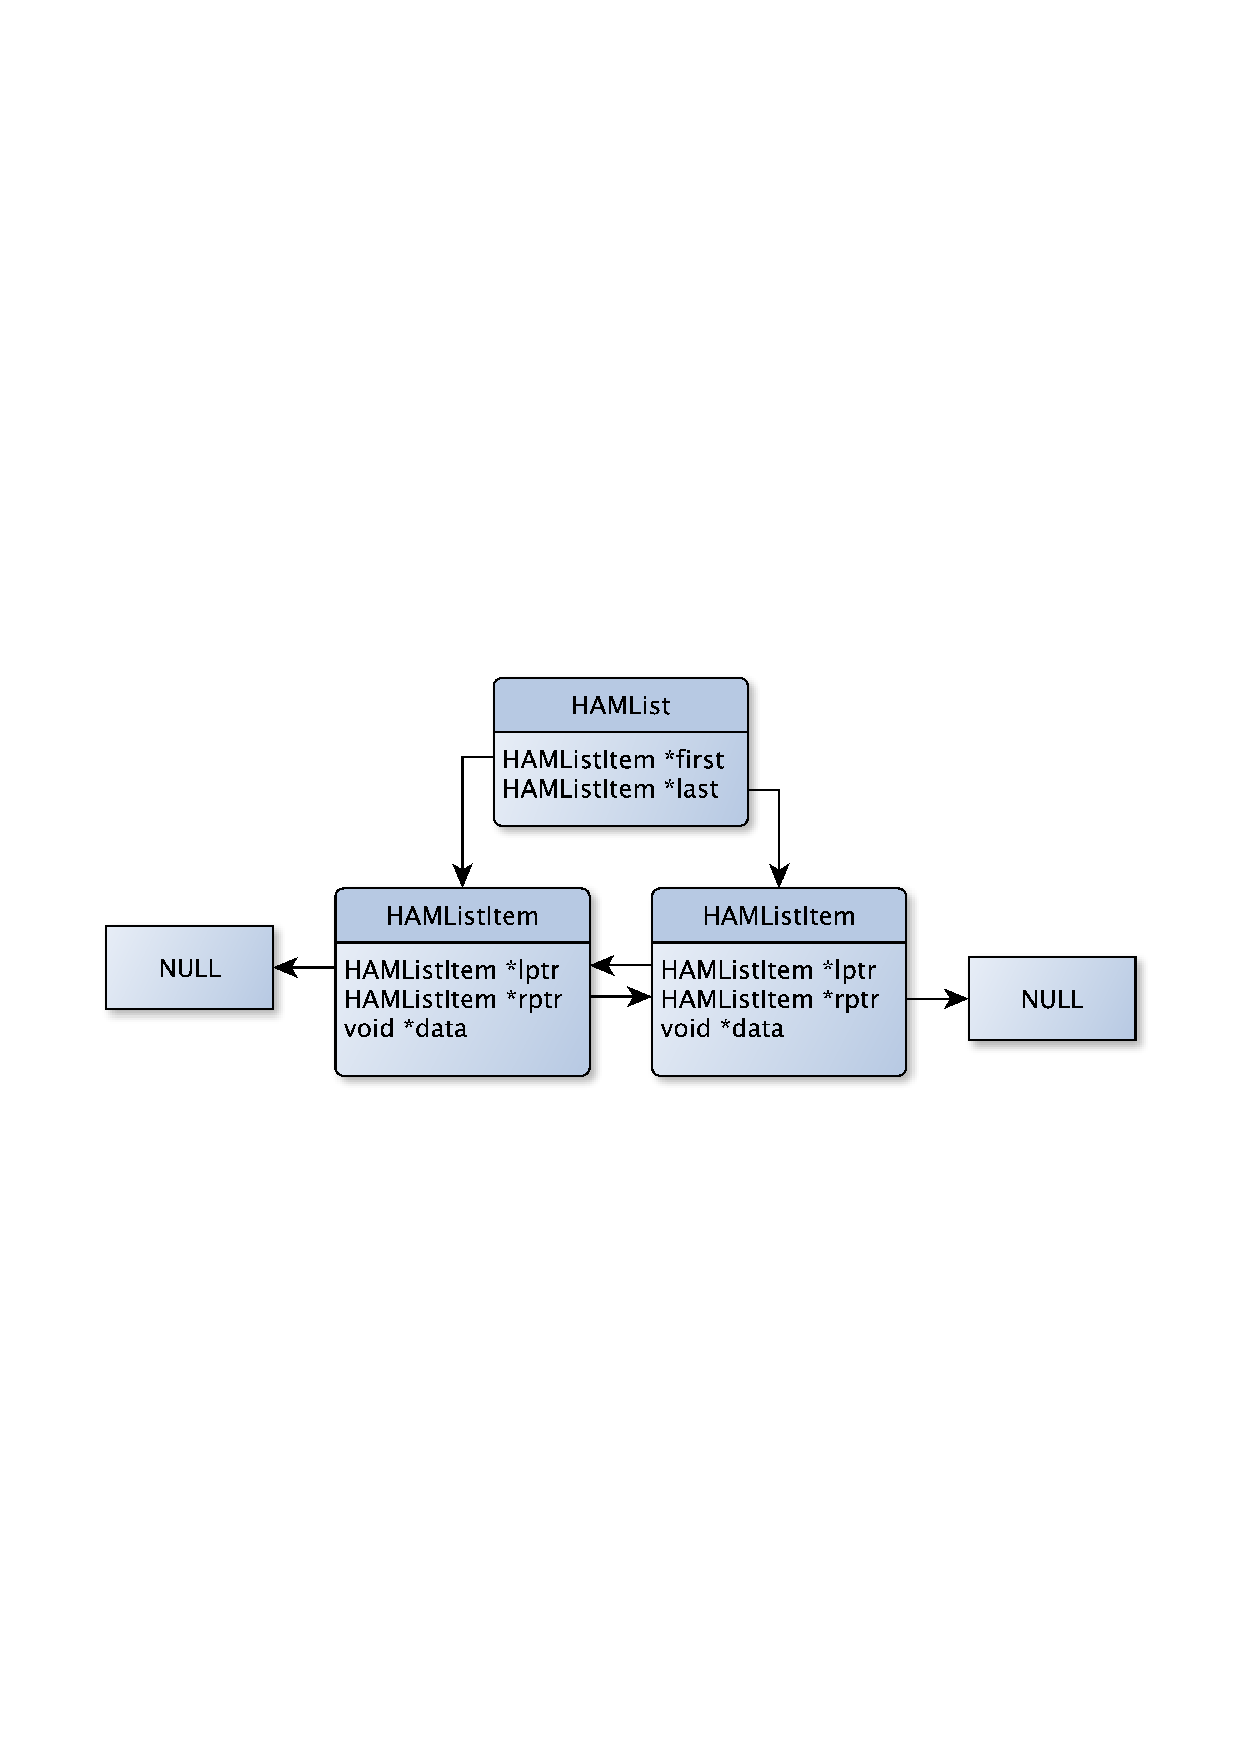
\includegraphics[trim=8cm 8cm 8cm 8cm, scale=0.6]{fig/list}
\caption{Diagram dvousměrného seznamu.}
\label{fig:hamlist}
\end{figure}

HAMList je implementací dvousměrného seznamu. Základní datové struktury použité pro definici seznamu jsou
HAMList a HAMListItem (viz obrázek \ref{fig:hamlist}):

\begin{verbatim}
typedef struct _HAMListItem {
	void *data;
	struct _HAMListItem *lptr;
	struct _HAMListItem *rptr;
} HAMListItem;

typedef struct _HAMList {
	HAMListItem *first;
	HAMListItem *last;
	HAMListItemDataFree free_func;
} HAMList;
\end{verbatim}

Každá položka HAMListItem obsahuje odkaz na svého předchůdce (lptr) a následníka (rptr) a samotná data spjatá
s položkou (data). Struktura HAMList obsahuje odkaz na první a poslední položku a ukazatel na funkci free\_func,
která je použita pro uvolnění uživatelských dat z paměti. Pokud není tato funkce definována, nejsou uživatelská
data při uvolňování seznamu z paměti uvolněna.

\subsubsection{HAMHashTable - Hashovací tabulka}
%% YARDA (DONE): opět dát to do kontextu, k čemu se to používá

Druhým abstraktním datovým typem používaným v klientské knihovně je hashovací tabulky (HAMHashTable).
Hlavním využitím hashovací tabulky je implementace signálů, kde slouží pro rychlé vyhledání
správného signálu podle jeho jména. Je také použita pro uchování seznamu modulů dostupných na serveru.

\begin{figure}[h]
\centering
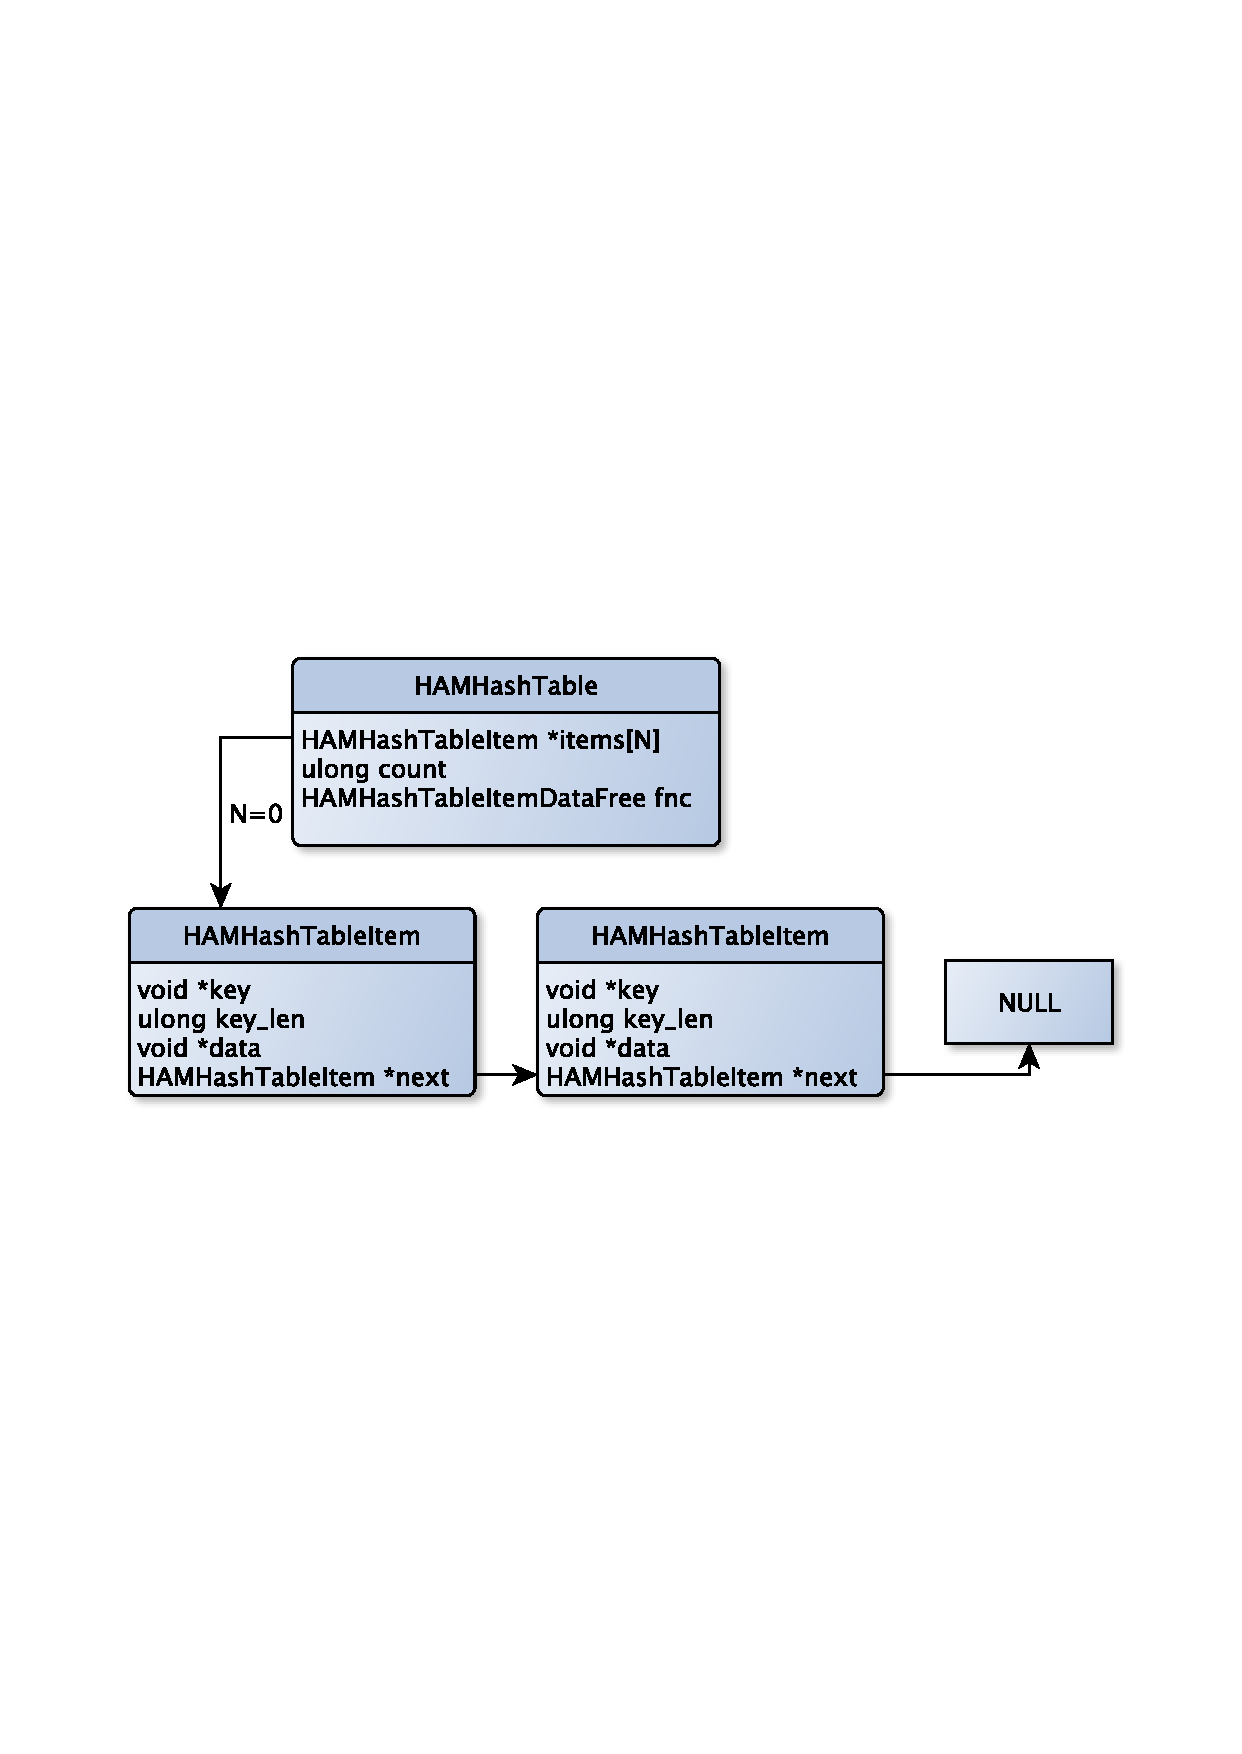
\includegraphics[trim=8cm 8cm 8cm 8cm, scale=0.6]{fig/hash}
\caption{Diagram hash tabulky seznamu.}
\label{fig:hamhashtable}
\end{figure}

HAMHashTable je implementací hash tabulky. Na obrázku \ref{fig:hamhashtable} lze vidět základní datové struktury
použíté při implementaci hash tabulky - HAMHashTableItem a HAMHashTable:

\begin{verbatim}
typedef struct _HAMHashTableItem {
	const void *key;
	void *data;
	unsigned long key_len;
	struct _HAMHashTableItem *next;
} HAMHashTableItem;

typedef struct _HAMHashTable {
	HAMHashTableItem *items[HAM_HASH_LEN];
	unsigned long count;
	HAMHashTableItemDataFree free_func;
} HAMHashTable;
\end{verbatim}

Každá položka uložená v hash tabulce obsahuje svůj klíč (key), jeho délku (key\_len), data svázaná s položkou a ukazatel
na další položku. Při vložení nové položky do tabulky je vypočten hash jejího kliče pomocí SDBM
hashovacího algoritmu \cite{sdbm}. %% YARDA: určitě link
Na základě hodnoty hashe je ukazatel na položku uložen do pole položek items.

\subsection{Komunikace s klientskou aplikací}
\label{implementace_knihovna_komunikace}

Pro komunikaci s klientskou aplikací je podstatné napojení na její smyčku událostí a možnost předávat asynchronně
výsledky požadavků odeslaných serveru. V této podkapitole jsou popsány řešení obou těchto problémů

\subsubsection{EventLoop}

Eventloop (neboli smyčka událostí) sdružuje metody sloužící k napojení na hlavní smyčku
klientské aplikace. Pro správnou funkci klientské
knihovny musí klientská aplikace implementovat všechny funkce definované ve struktuře HAMEventLoopUICallbacks a
předat je klientské knihovně prostřednictvím metody ham\_eventloop\_set\_ui\_callbacks().

Funkce definované ve struktuře HAMEventLoopUICallbacks jsou pak používány dalšími částmi klientské knihovny na
následující činnosti:

\begin{itemize}
\item timeout\_add - Přidá do hlavní smyčky aplikace běžící v klientské aplikaci
nový časovač. Klientská aplikace
musí vrátit ukazatel na strukturu jednoznačně identifikující časovač a
volat opakovaně ve zvoleném intervalu funkci předanou jako ukazatel.
\item timeout\_remove - Odebere z hlavní smyčky časovač na základě ukazatele na strukturu, která jej identifikuje.
\item input\_add - Přidá do hlavní smyčky klientské aplikace ukazatel na funkci, která je volána když jsou k dispozici
nová data na definovaném soketu. Klientská aplikace
musí vrátit ukazatel na strukturu jednoznačně identifikující tuto událost.
\item input\_remove - Odebere z hlavní smyčky ukazatel na funkci vstupu na
základě ukazatele na strukturu, která jej identifikuje.
\end{itemize}

Díky této abstrakci je tak možno napojit klientskou knihovnu na jakoukoliv smyčku událostí.

\subsubsection{Signály}

Jednotlivé části klientské knihovny umožňují definovat signály, na které se pak může klientská aplikace napojit.
Seznam signálů je uložen v hash tabulce, kde klíčem je název signálu a daty seznam funkcí, které jsou zavolány
pokud je signál emitován. K registraci nových signálů slouží funkce ham\_signals\_register\_signal().

Klientské aplikaci je umožněno funkcí ham\_signals\_register\_handler() zaregistrovat funkci, která je zavolána
při emitování signálu. Funkce musí být ve formátu HAMFetchHandler. Při registraci signálu lze rovněž definovat
ukazatel na data, která jsou při emitování signálu zpracovávající funkci předána. Toho lze využít pro udržování
kontextu při zpracovávání signálu.


\subsection{Komunikace se serverem}

Tato podkapitola popisuje implementaci komunikace se serverem v klientské knihovně. Je zde popsáno rozhraní pro
připojení k serveru, parser komunikačního protokolu a pomocné struktury HAMRequest a HAMReply pro reprezetanci odchozích a
příchozích paketů.

\subsubsection{Připojení k serveru}

Pro připojení k serveru je nutné vytvořit novou instanci struktury Connection funkcí ham\_connection\_new(). Touto funkcí
se definuje adresa a port serveru, uživatelské jméno a heslo. Samotné připojení proběhne až po zavolání funkce
ham\_connection\_connect(). Tato funkce vytvoří nový soket pro připojení k serveru a pomocí funkce ham\_eventloop\_input\_add()
přidá do hlavní smyčky aplikace ukazatel na funkci pro parsování přijatých dat.

\subsubsection{Odeslání požadavku}

Požadavek je reprezentován strukturou HAMRequest. Její instanci lze vytvořit metodou ham\_request\_new(). Lze určit
URI, na které bude požadavek zaslán, typ požadavku (GET nebo POST) a zasílaná data. Samotný požadavek pak lze odeslat
metodou ham\_connection\_send() (případně ham\_connection\_send\_destroy(), která jej i uvolní z paměti).

Pro použití standardních modulů jsou však v klientské knihovně implementovány jednoduché metody, které vytváření a odesílání
požadavků provádějí automaticky. Rovněž jsou definovány signály pro zpracování odpovědí na tyto standardní dotazy.
V praxi tak stačí aplikaci využívající klientskou knihovnu zavolat například metodu ham\_dxcc\_fetch(), která odešle
potřebný požadavek serveru a při přijetí odpovědi automaticky emituje signál, na který se může klienstká aplikace napojit.

\subsubsection{Parsování odpovědi}

K parsování dat v klientské knihovně slouží HAMParser. Ten funguje na stejném principu jako RequestParser na straně serveru.
Parsovaná data jsou ukládána do struktury HAMReply, která pak předána prostřednictvím signálu nebo zpětného volání (callbacku)
funkci, která požadavek na server iniciovala.

\section{Klientská aplikace}
\label{implementace_klient}

Referenční klientská aplikace byla naprogramována v jazyce C++ s využitím grafického frameworku Qt \cite{qt}. V této kapitole jsou stručně
popsány jednotlivé části klientské aplikace, třídy, které klientskou aplikaci implementují a jejich napojení na klientskou knihovnu.

\subsection{Hlavní okno aplikace}

V této podkapitole je popsána implementace hlavního okno aplikace (znázorněno na obrázku \ref{fig:okno}) a všech prvků, které jej tvoří.

\begin{figure}[h]
\centering
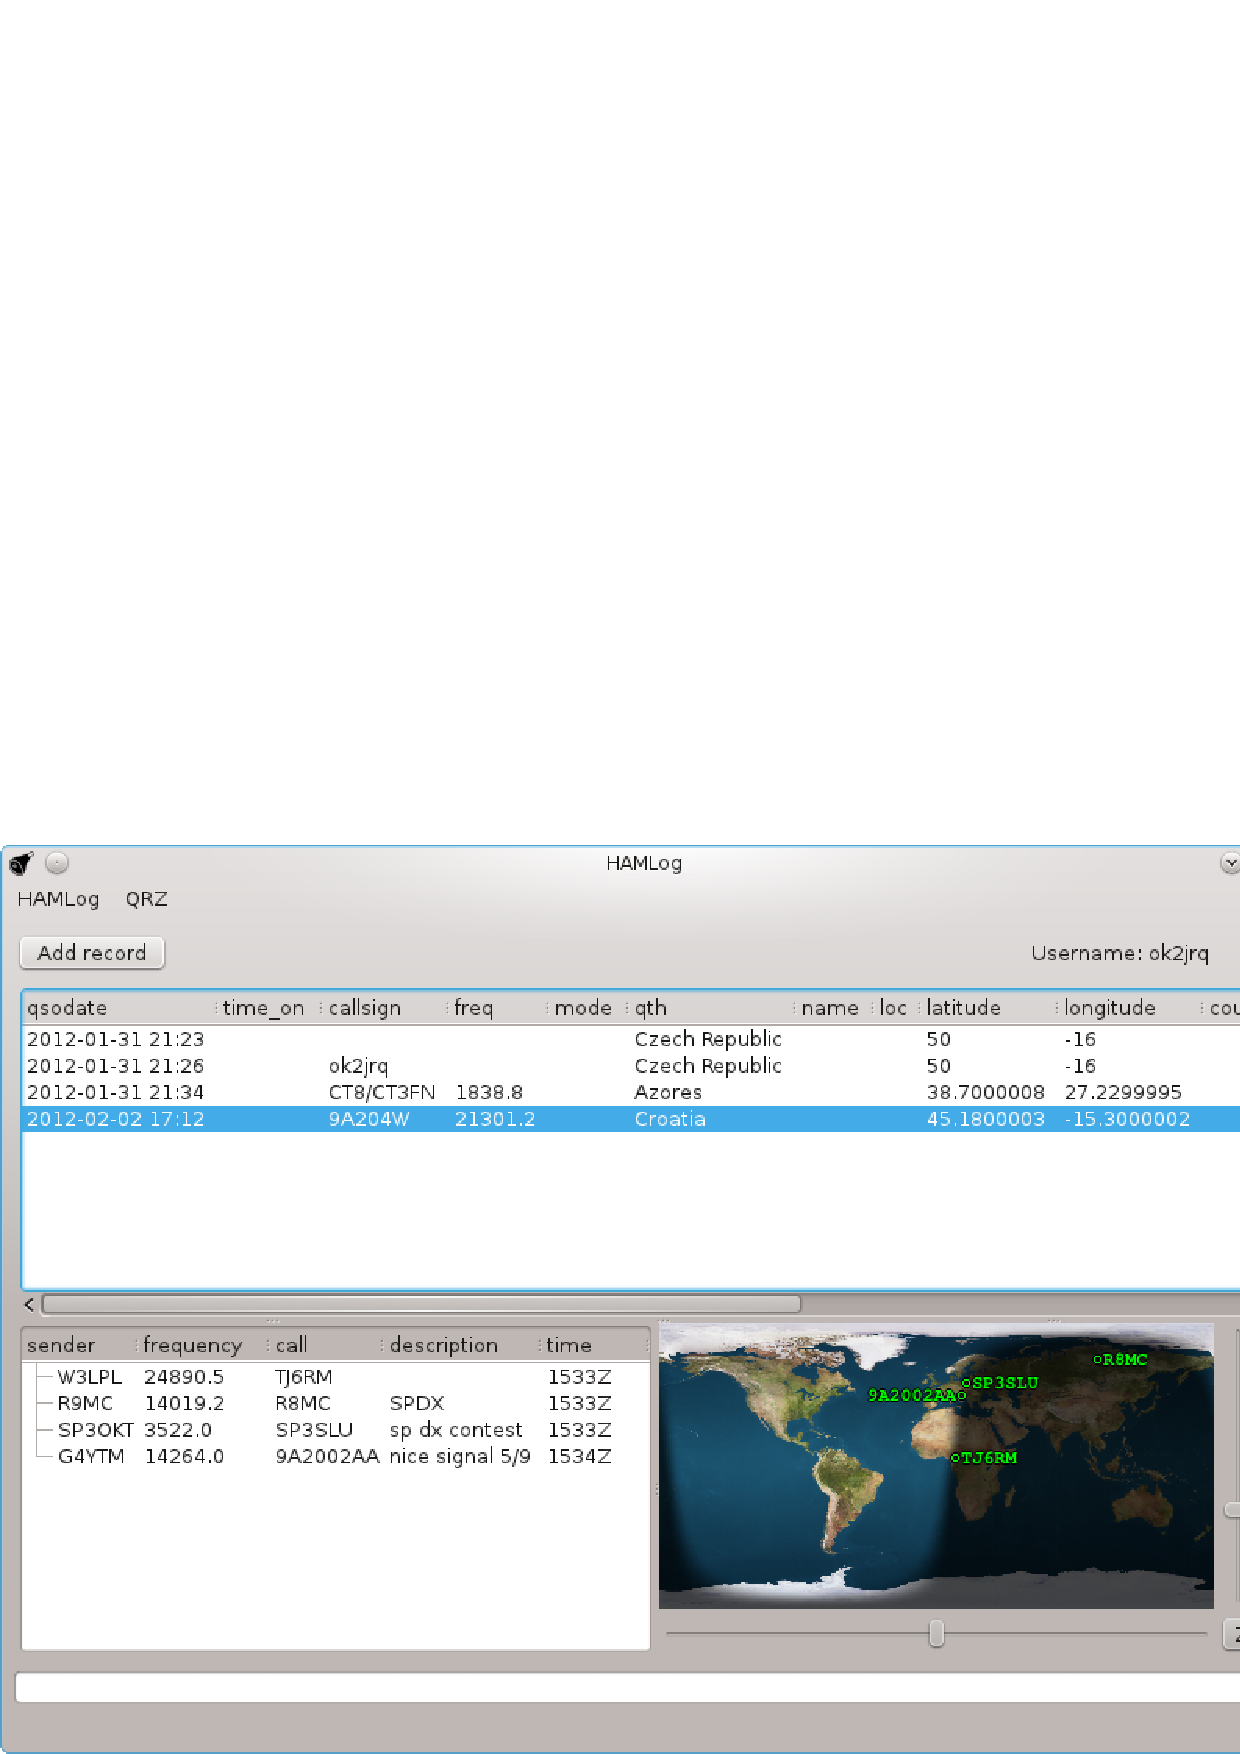
\includegraphics[trim=0cm 0cm 0cm 0cm, scale=0.7]{fig/ham3}
\caption{Hlavní okno aplikace.}
\label{fig:okno}
\end{figure}

\subsubsection{Třída MainWindow}

Třída MainWindow reprezentující hlavní okno je také hlavní třídou klientské aplikace. Po svém vytvoření zobrazí dialog
pro připojení uživatele k serveru. Pomocí metody connectServer() se pak přihlásí
k serveru. Nový uživatelský
účet se registruje metodou registerAccount.

Třída MainWindow se o úspěšném, případně neúspěšném přihlášení k serveru dozví díky napojení
na patřičné signály klientské knihovny. V této třídě je také implementována komunikace mezi jednotlivými prvky tvořícími hlavní okno
prostřednictvím Qt signálů.

\subsubsection{Třída LogbookTreeWidget}

Třídou LogbookTreeWidget je uživateli umožněno zobrazení a editace logu prostřednictvím rozhraní podobného tabulce.
Je implementována nad Qt třídou QTreeWidget a komunikuje 
se serverovým modulem Logbook prostřednictvím klientské knihovny. Jednotlivé položky jsou editovatelné a změny se přenášejí
na server. Pokud uživatel poklepe na některou z položek, je zpracován příslušný Qt signál a otevřen dialog NewRecordDialog,
ve kterém může uživatel položku také editovat.

\subsubsection{Třída EarthWidget}

Třída EarthWidget je technologicky nejzajímavější třídou klientské aplikace. Umožňuje zobrazit zeměkouli promítnutou do roviny i 
formou klasického globusu (obrázek \ref{fig:globus}). Na zeměkouli lze pak zobrazovat značky s popisky. Toho je využito pro zobrazení polohy právě vysilájících
stanic.

\begin{figure}[h]
\centering
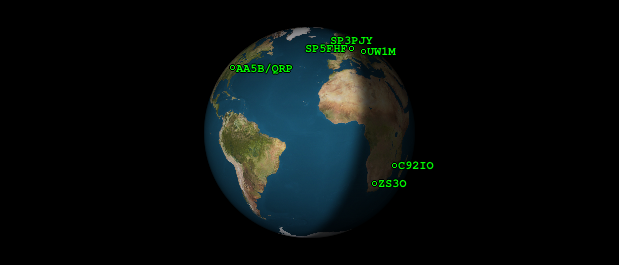
\includegraphics[trim=0cm 0cm 0cm 0cm, scale=0.9]{fig/ham5}
\caption{Ukázka možnosti zobrazení zeměkoule.}
\label{fig:globus}
\end{figure}

Pro zobrazení zeměkoule je využita aplikace Xplanet. Při požadavku na překreslení okna je spuštěn nový proces Xplanet
s požadovanými parametry a je mu předáno ID widgetu, do kterého má vykreslovat. Značky s popisky jsou uloženy do dočasného souboru
a tento soubor je pak načten aplikací Xplanet a použit k vykreslení značek.
EarthWidget umožňuje také přiblížení na předdefinované lokace (například přiblížení Evropy) pomocí kontextového menu.

\subsubsection{Třída DXClusterWidget}

Pomocí třídy DXClusterWidget je zobrazen seznam aktuálně vysílajících stanic. Třída se prostřednictvím klientské knihovny
v pravidelných intervalech dotazuje
serveru na seznam aktuálně vysílajících stanic a tento pak zobrazuje. Pokud uživatel na některou ze stanic poklepe, otevře se 
dialog pro přidání nového záznamu. Seznam stanic je také předáván za pomoci Qt signálu třídě EarthWidget, která pak stanice
vykresluje na mapě.

\subsection{Přidání nového záznamu a editace}

Nový záznam lze přidat dvěma způsoby. Buď tak lze učinit pomocí tlačítka "Add Record" v hlavním okně aplikace, nebo poklepáním
na stanici získanou z DXClusteru. Obě možnosti pak vedou k vyvolání dialogu pro přidání nového záznamu
(zobrazen na obrázku \ref{fig:novy_zaznam}). Stejný dialog je použit
také pro editaci již existujícího záznamu. Editaci lze vyvolat poklepáním na existující záznam v hlavním okně aplikace.

\begin{figure}[h]
\centering
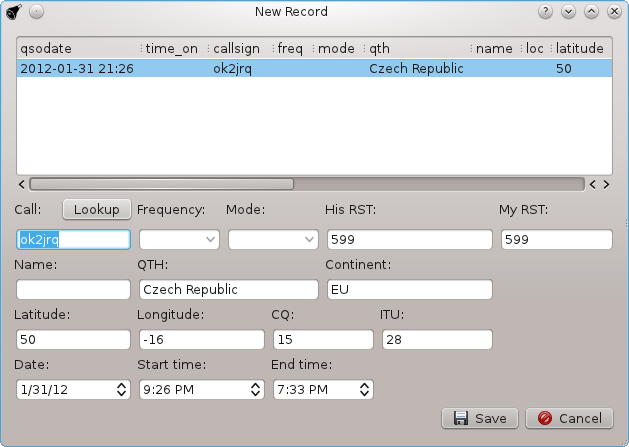
\includegraphics[trim=0cm 0cm 0cm 0cm, scale=0.9]{fig/ham4}
\caption{Dialog pro přidání a editaci záznamu.}
\label{fig:novy_zaznam}
\end{figure}

\subsubsection{Třída NewRecordDialog}

Dialog pro přidání nového záznamu a jeho editaci je implementován v třídě NewRecordDialog. Dialog se skládá ze dvou částí:

\begin{itemize}
\item Tabulka zobrazující předchozí spojení s přidávanou stanicí.
\item Formulář s jednotlivými poli o nově přidávaném záznamu.
\end{itemize}

Pro implementaci tabulky s předchozími spojeními je použita třída
LogbookTreeWidget. Je tak znovu použit již jednou vytvořený
kód.

V případě změny pole pro zadání volací značky (Call sign), je aktualizována tabulka s historií, a uživatel tak vidí předešlá 
spojení s danou stanicí. Také se pomocí klientské knihovny zjistí podrobné informace o zadané stanici a předvyplní se patřičná
pole. To zrychluje zadávání nových záznamu. V případě změny hodnoty v poli frekvence je na server odeslán požadavek o přeladění
radiostanice na zadanou frekvenci.
%% YARDA (DONE: pridano k popisu modulu hamlib): někde do textu dát, že komunikace s radiostanicí byla prakticky
%% vyzkoušena s radiostanici ICOM IC-706MKIIG (taky důležité)

Po potvrzení dialogu jsou hodnoty všech polí prostřednictvím klientské knihovny přeneseny na server, kde jsou uchovány.

\subsection{Zobrazení dostupných modulů}

Dialog zobrazující moduly dostupné na serveru (viz obrázek \ref{fig:moduly_dialog}) lze spustit prostřednictvím hlavního menu aplikace.

\begin{figure}[h]
\centering
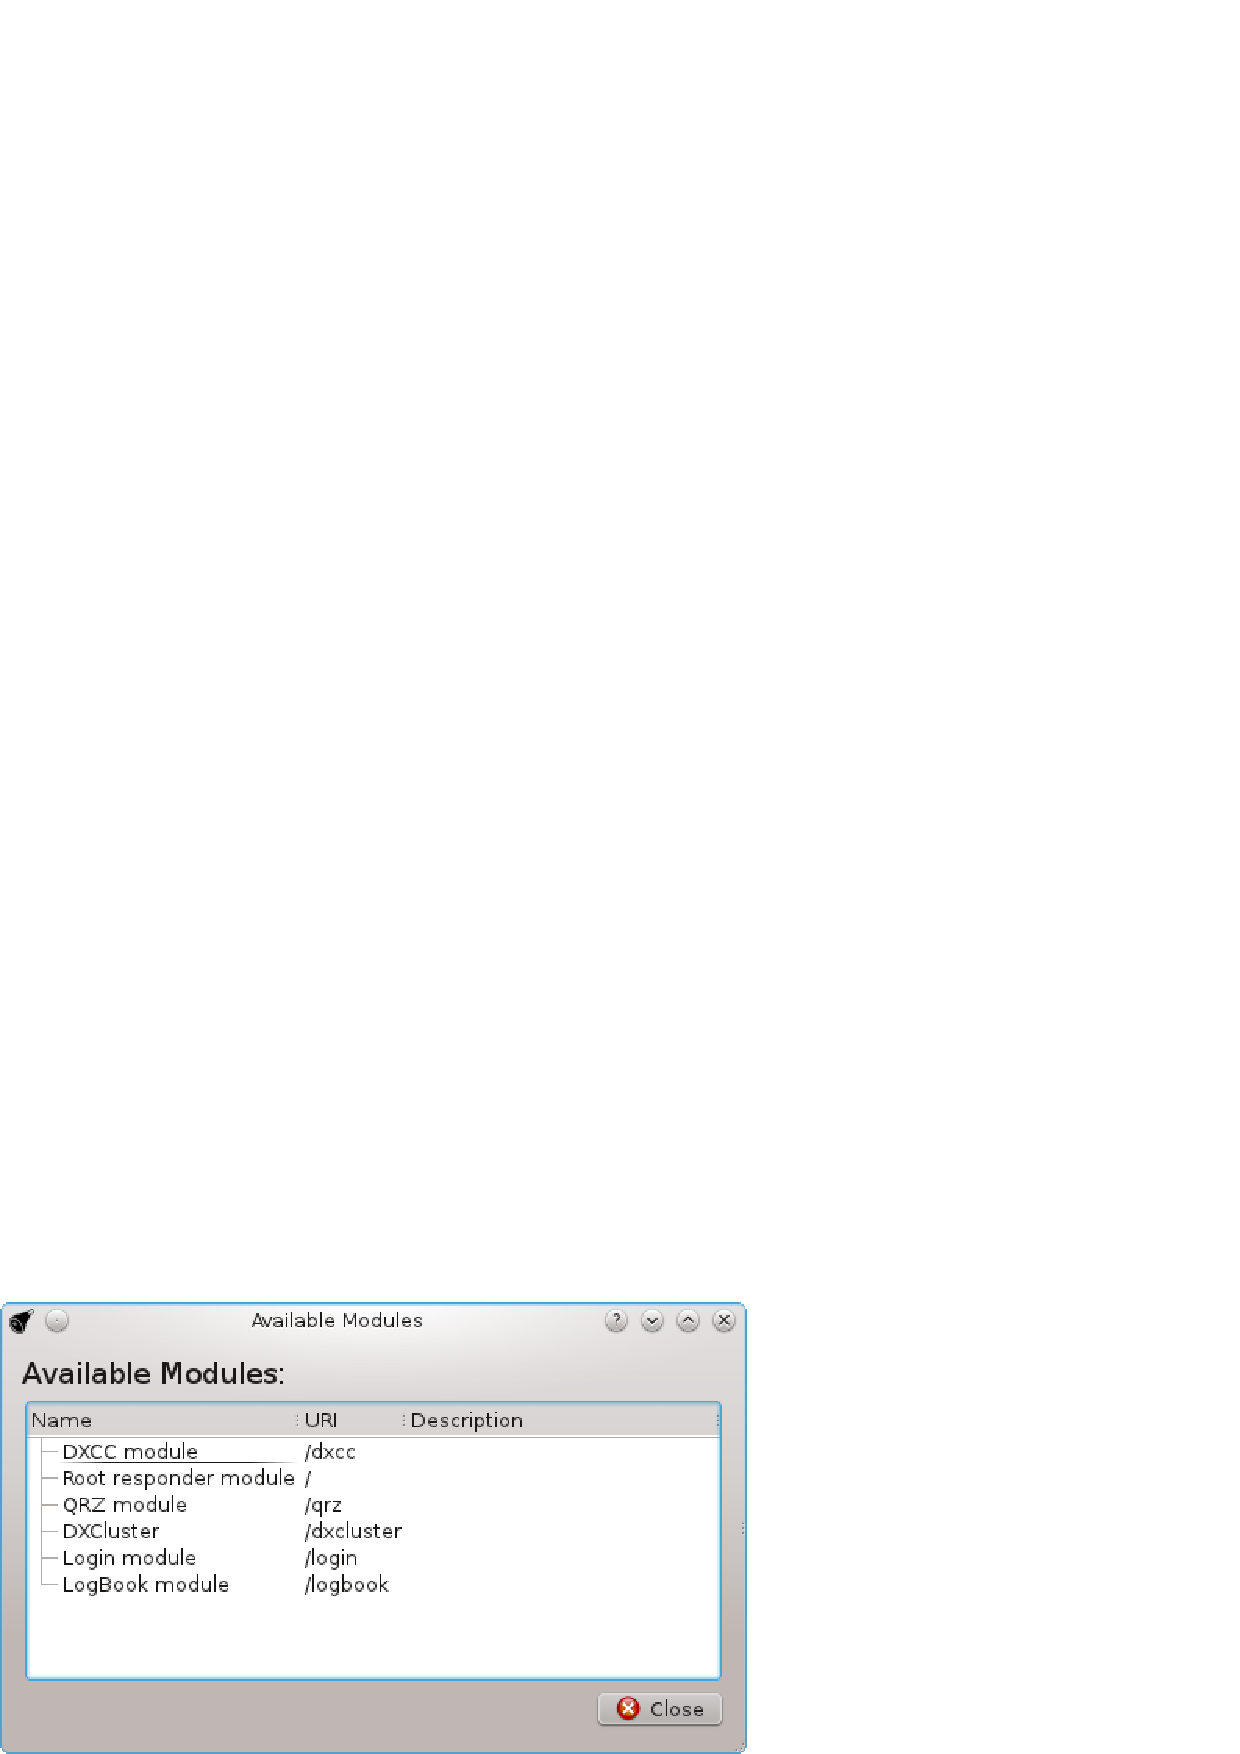
\includegraphics[trim=0cm 0cm 0cm 0cm, scale=1]{fig/ham6}
\caption{Dialog zobrazující dostupné moduly.}
\label{fig:moduly_dialog}
\end{figure}

\subsubsection{Třída NewRecordDialog}

Dialog zobrazující dostupné moduly je implementován třídou NewRecordDialog. Jedná se o jednoduchou třídu, která pomocí
klientské knihovny získá ze serveru seznam modulů a zobrazí je formou tabulky vytvořené díky Qt widget QTreeWidget.

\chapter{Ukázka použití aplikace}

V této kapitole je stručně popsáno typické použití aplikace na jednoduchém příkladu.

Po přihlášení k serveru vidí operátor radiostanice hlavní okno aplikace (obrázek \ref{fig:okno}).
V tomto hlavním okně se po chvíli začnou v jeho dolní části zobrazovat ostatní radioamatéři, kteří
právě vysílají (DX Cluster). Operátor má možnost vidět na mapě světa umístění těchto stanic. Pro získání většího 
detailu lze mapu světa přiblížit na požadovanou oblast. Může také změnit zobrazení a zobrazit klasický
globus (obrázek \ref{fig:globus}).

Pokud se operátor rozhodne začít komunikaci s některým s dalších vysílajících radioamatérů, stačí
poklepat na jeho volací značku v seznamu a dojde k otevření dialogového okna pro navázaní nového spojení (obrázek \ref{fig:novy_zaznam}).
Otevřením dialogového okna se pomocí serveru QRZ.COM a DXCC databáze získají další detailní informace o radioamatérovi, se kterým 
se operátor snaží navázat spojení. V tento moment se také automaticky přeladí radiostanice připojená
k jeho počítači a on může začít zkoušet navázat spojení.

V tomto okně lze také vidět předešlá spojení s tímto radioamatérem a operátor se tak může rozhodnout, zda-li chce
navázat spojení s někým, s kým už se v minulosti spojil.

Během komunikace vyplní operátor další požadované údaje jako například přijatý a odeslaný RST report. Jakmile je komunikace
u konce, uzavře operátor dialogové okno pro přidání nového záznamu a spojení se zapíše do deníku.

Pokud se operátor v budoucnu rozhodne záznam o spojení upravit (například za účelem změny příznaku o 
přijatém QSL lístku), lze jednoduše poklepat na spojení a editovat ho ve stejném dialogu jako při jeho
přidání.

\chapter{Závěr}
Cílem této bakalářské práce bylo navhrnout a implementovat softwarovou aplikaci
pro vedení staničního deníku určeného pro operátory amatérské radiokomunikační služby. Důraz byl kladen zejména
na modularitu a otevřenost návrhu. Pro úspěšné dokončení práce bylo nutné se
seznámit se 
základními principy, aplikacemi a terminologií používanou radiamatéry.
Bylo nutné se zorientovat v 
radioamatérské technologii a pochopit fungování celého radioamatérského společenství.
Výsledný návrh se snaží odstranit problémy jimiž trpí v současné době dostupné
aplikace a zaplnit volné místo mezi aplikacemi umožňujícími vedení staničního deníku.

Výstupem implementace jsou tři oddělené projekty (serverová aplikace, klientská knihovna a grafické uživatelské rozhraní),
které spolu spolupracují a vzájemně se doplňují.

Serverová aplikace je plně modulární a umožňuje jednoduché přidávání nových
funkcí pomocí modulů. Splňuje veškeré požadavky na základní vedení staničního deníku (přidávání/editace záznamů, vyhledávání 
informací o ostatních radioamatérech nebo například ovládání vysílačky připojené k počítači).

Pokud serverová aplikace poběží na skutečném serveru, je díky systému modulů
možné např. jednoduše vytvořit modul
pro generování deníku na webové stránky. Případně, díky využití protokolu kompatibilního s protokolem HTTP, použít rovnou
serverovou aplikaci jako jednoduchý webový server.
%% YARDA (DONE): vypíchnout, že se to může použít např. pro automatické generování logu
%% na WWW stránky, atp.

Klientská knihovna je důležitým prvkem implementace, protože implementuje nízkoúrovňovou komunikaci s serverovou aplikací
a umožňuje tak grafickému uživatelskému rozhraní zaměřit se pouze na komunikaci s uživatelem. Klientskou knihovnu
je možné použít pro jednodušší tvorbu klientských aplikací a v budoucnu se předpokládá vznik dalších specializovaných
klientských aplikací například pro zapisování spojení z terénu prostřednicvím mobilního telefonu.

%% YARDA (DONE): opět vypíchnout, že se předpokládá vznik dalších klientů, např. pro
%% mobil pro logování z terénu
Grafické uživatelské není přiliš rozsáhlé, ale umožňuje vést staniční deník pohodlně a poskytuje všechny základní funkce potřebné
pro vedení staničního deníku. Je graficky přehledné a pro stávající radioamatéry intuitivní.

Celkově je výsledná aplikace dobrým základem pro implementaci dalších nadstandardních funkcí. Byla uvolněna pod licencí
GPL a je k dispozici na webu Githubu. Během vývoje byla aplikace konzultována se skutečnými radioamatéry, kteří rovněž
přislíbili účast na dalším vývoji. V budoucnu je pak v plánu integrace aplikace
do nejpoužívanějších linuxových distribucí (balíčky RPM, DEB, ebuild, \ldots).

%% YARDA (DONE): pochlubit se, že se jedná o opensource projekt uvolněný pod GPL, který
%% je k dispozici na githubu (link), bude zabalen do fedory a už má svoje příznivce
%% :) takže se základna vývojářů určitě rozšíří

\section{Možnosti budoucího rozšíření}

Během implementace a testování aplikace vyplynuly některé další možnosti, jakým směrem aplikaci v budoucnu rozšiřovat.

\subsection{Podpora MySQL}

Pro standardní použití jedním uživatelem je databázový systéme SQLite3 zcela jistě dostačující.
Pro větší nasazení s více uživateli využívajícími funkce serveru současně by však bylo vhodné implementovat podporu pro databázový
systém MySQL. Přidat podporu pro jinou databázi je díky současnému návrhnu jednoduché.
%% YARDA (tak na pul DONE): možná se zmínit, že v
%% současnosti používané use cases nepředpokládají vysoké zatížení, takže to v
%% současnosti dostačuje, ale, že třeba by se to hodilo pro multiops, což je oblast
%% dosud neprozkoumaná, protože podobný produkt neexistuje

\subsection{Moduly pro tvorbu statistik}

Dalším možným rozšířením je implementace modulů umožňujících generování statistik a přehledů o jednotlivých záznamech v deníku.
Uživateli tyto moduly umožní lepší orientaci v jeho deníku a na straně serveru je pak možné generovat žebříček uživatelů na
základě různých klíčů, snadno zobrazovat bodu získáné v soutěžích v reálném čase nebo například generovat diplomy
(DXCC, IOTA, SOTA).

Díky zvolenému návrhu a implementaci databázového rozhraní lze konstruovat kompletní dotazy pro databázi a lze tedy získat
data pro nepřeberné množství statistik. Navíc je díky implementaci modulů serveru jednoduché tyto nové funkce přidávat,
protože nikdy nejsou součástí jádra aplikace, ale pouze toto jádro rozšiřují.
%% YARDA (DONE): více rozvést, že lze konstruovat kompletní dotazy a tedy spočítat
%% statistiky prakticky pro cokoliv, a že lze snadno zobrazovat body získané v
%% jednotlivých soutěžích, závodech a diplomech (např. DXCC, IOTA, SOTA, atp.).


 % viz. obsah.tex

  % Pouzita literatura
  % ----------------------------------------------
\ifczech
  \bibliographystyle{czechiso}
\else 
  \bibliographystyle{plain}
%  \bibliographystyle{alpha}
\fi
  \begin{flushleft}
  \bibliography{projekt} % viz. literatura.bib
  \end{flushleft}
  \appendix
  
  %\chapter{Obsah CD}
%\chapter{Manual}
%\chapter{Konfigra�n� soubor}
%\chapter{RelaxNG Sch�ma konfigura�n�ho soboru}
%\chapter{Plakat}

 % viz. prilohy.tex
\end{document}
